\documentclass[12pt,a4paper]{report}
\usepackage[utf8]{inputenc}
\usepackage[T1]{fontenc}
\usepackage[a4paper, top=2.5cm, bottom=2.5cm, left=3.5cm, right=2.5cm]{geometry}
\usepackage{graphicx}
\usepackage{hyperref}
\usepackage{booktabs}
\usepackage{array}
\usepackage{listings}
\usepackage{xcolor}
\usepackage{setspace}
\usepackage{fancyhdr}
\usepackage{float}
\usepackage{amsmath}
\usepackage{caption}
\usepackage{parskip}
\usepackage{enumitem}
\usepackage{multirow}
\usepackage{tabularx}
\usepackage{tikz}
\usepackage{pgfplots}
\usepackage{times}
\usepackage{titlesec}

\pgfplotsset{compat=1.18}
\usetikzlibrary{arrows.meta, shapes.geometric, positioning}

\hypersetup{colorlinks=false, pdfborder={0 0 0}}
\doublespacing

% ---- Bölüm/alt bölüm başlık biçimi ----
\titleformat{\chapter}[hang]
  {\normalfont\large\bfseries\centering}
  {\thechapter.~}{0pt}{}
\titlespacing*{\chapter}{0pt}{-10pt}{20pt}

\titleformat{\section}[hang]
  {\normalfont\normalsize\bfseries}{\thesection.}{0.5em}{}
\titleformat{\subsection}[hang]
  {\normalfont\normalsize\bfseries}{\thesubsection.}{0.5em}{}

% ---- Sayfa stili ----
\pagestyle{fancy}
\fancyhf{}
\fancyhead[R]{\thepage}
\renewcommand{\headrulewidth}{0pt}
\fancypagestyle{plain}{\fancyhf{}\fancyhead[R]{\thepage}\renewcommand{\headrulewidth}{0pt}}

% ---- Kod listeleri ----
\lstset{
  basicstyle=\footnotesize\ttfamily,
  breaklines=true,
  frame=single,
  backgroundcolor=\color{gray!10},
  keywordstyle=\color{blue},
  commentstyle=\color{green!50!black},
  stringstyle=\color{red!60!black},
  numbers=left,
  numberstyle=\tiny\color{gray},
  numbersep=5pt
}

% =============================================================
\begin{document}
\pagenumbering{roman}

% ===================== KAPAK SAYFASI =========================
\begin{titlepage}
\thispagestyle{empty}
\centering
\vspace*{2cm}
{\large\bfseries
SMART WASTE MANAGEMENET SYSTEM
(ECOHAUL)\par}
\vspace{4cm}
{\normalsize by
\\[0.4cm]}
{\large\bfseries Atahan Düryaz\par}
\vspace{4cm}
{\large\bfseries Engineering Project Report
\par}
\vspace{3cm}
{\normalsize
Yeditepe University\\
Faculty of Engineering\\
Department of Computer Engineering\\
2026\par}
\end{titlepage}

\clearpage\thispagestyle{empty}\phantom{x}\clearpage
\setcounter{page}{2}

% ===================== ONAY SAYFASI ==========================
\thispagestyle{plain}
\begin{center}
{\large\bfseries
SMART WASTE MANAGEMENET SYSTEM (ECOHAUL)\par}
\end{center}
\vspace{2cm}
\noindent APPROVED BY::
\vspace{1.2cm}

\noindent Prof. Dr. \c{S}ebnem Baydere \dotfill\\
(Supervisor)

\vspace{0.9cm}
\noindent Prof. Dr. Gürhan Küçük \dotfill\\


\vspace{0.9cm}
\noindent  Dr. Öğr. Üyesi Esin Onba\c{s}{\i}o\u{g}lu \dotfill\\


\vfill
\noindent DATE OF APPROVAL:03/06/2026
\clearpage

% ===================== TEŞEKKÜR =============================
\chapter*{ACKNOWLEDGEMENTS}
\addcontentsline{toc}{chapter}{ACKNOWLEDGEMENTS}

\indent First of all, I would like to thank my advisor Prof.\ Dr.\ \c{S}ebnem Baydere for her support, guidance,
and discipline throughout my project. In addition, I would like to thank our assistants for
their support whenever I needed help.

In addition, I would like to thank my parents, my friends, and my cat for their support and encouragement throughout the process. They always made me feel their support and put effort into my education.

In memory of Atakan DÜRYAZ. 




\clearpage
% ===================== ABSTRACT ==============================
\chapter*{ABSTRACT}
\addcontentsline{toc}{chapter}{ABSTRACT}

\begin{center}
{\large\bfseries SMART WASTE MANAGEMENT SYSTEM FOR URBAN ENVIRONMENTS (EcoHaul)}
\end{center}
\vspace{0.8cm}

\indent This project presents the design and implementation of EcoHaul, an AI-driven smart waste management system for urban environments. The system employs a parallel dual-world simulation architecture to compare a novel Dynamic Priority and Efficient Truck dispatch (DPET) algorithm against a traditional fixed-route approach across 3,424 real waste bin locations sourced from the Dublin City Council open dataset. Two independent simulation worlds run concurrently under identical environmental conditions, ensuring that any observed performance difference is attributable solely to the dispatch strategy.

\indent The DPET algorithm integrates a six-layer processing pipeline comprising traffic modeling, bin priority scoring, bin selection, mass-aware route optimization, route efficiency validation, and truck dispatching. A K-means clustering-based fill predictor with Estimated Time to Full (ETF) learning enables proactive dispatch decisions before bins overflow. The system further incorporates an urban environment model that simulates district-specific fill-rate behaviors driven by morning office rushes, evening mall peaks, and stochastic civic events such as concerts, matches, and festivals.

\indent A React-based interactive dashboard with Leaflet mapping provides real-time visualization of bin states, truck movements, anomaly events, and comparative key performance indicators. An IoT integration layer supports ESP32 microcontrollers paired with JSN-SR04T waterproof ultrasonic sensors for physical deployment alongside the simulation. Experimental results from 30-day simulations demonstrate that DPET achieves 26.6\% fuel savings, 75\% fewer overflow events, and a 24.1\% cost reduction compared to fixed-route collection, while an anomaly detection subsystem identifies six categories of operational and sensor anomalies with an overall accuracy of 97.6\%.

\clearpage
% ===================== ÖZET ==================================
\chapter*{ÖZET}
\addcontentsline{toc}{chapter}{ÖZET}

\begin{center}
{\large\bfseries KENTSEL \c{C}EVRELERDE AKILLI ATIK Y\"ONET\.{I}M S\.{I}STEM\.{I} (EcoHaul)}
\end{center}
\vspace{0.8cm}

\indent Bu proje, kentsel \c{c}evreler i\c{c}in yapay zeka destekli bir ak\i{}ll\i{} at\i{}k y\"onetim sistemi olan EcoHaul'un tasar\i{}m\i{}n\i{} ve uygulamas\i{}n\i{} sunmaktad\i{}r. Sistem, Dublin Belediyesi a\c{c}\i{}k veri setinden elde edilen 3.424 ger\c{c}ek at\i{}k konteyneri konumu \"uzerinde, yeni bir Dinamik \"Oncelik ve Verimli Kamyon Sevk (DPET) algoritmas\i{}n\i{} geleneksel sabit g\"uzerg\^ah yakla\c{s}\i{}m\i{}yla kar\c{s}\i{}la\c{s}t\i{}rmak amac\i{}yla paralel \c{c}ift d\"unya sim\"ulasyon mimarisini kullanmaktad\i{}r. Bu mimaride iki ba\c{g}\i{}ms\i{}z sim\"ulasyon d\"unyas\i{} \"ozde\c{s} \c{c}evresel ko\c{s}ullar alt\i{}nda e\c{s} zamanl\i{} \c{c}al\i{}\c{s}t\i{}r\i{}larak, g\"ozlemlenen her performans fark\i{}n\i{}n yaln\i{}zca sevkiyat stratejisine atfedilebilmesi sa\u{g}lan\i{}r.

\indent DPET algoritmas\i{}; trafik modellemesi, konteyner \"oncelik puanlamas\i{}, konteyner se\c{c}imi, k\"utle bilin\c{c}li g\"uzerg\^ah optimizasyonu, g\"uzerg\^ah verimlilik do\u{g}rulamas\i{} ve kamyon sevkiyat\i{}n\i{} kapsayan alt\i{} katmanl\i{} bir i\c{s}leme hatt\i{}n\i{} entegre etmektedir. Tahmini Dolma Zaman\i{} (TDZ) \"o\u{g}renmesiyle desteklenen K-ortalamalar k\"umeleme tabanl\i{} dolma tahmincisi, konteynerler dolup ta\c{s}madan \"once proaktif sevkiyat kararlar\i{} al\i{}nmas\i{}n\i{} m\"umk\"un k\i{}lar. Sistem ayr\i{}ca sabah ofis yo\u{g}unlu\u{g}u, ak\c{s}am al\i{}\c{s}veri\c{s} merkezi tepe saatleri ve konser, ma\c{c}, festival gibi rastgele sivil etkinliklere dayal\i{}, b\"olgeye \"ozg\"u dolma h\i{}z\i{} davran\i{}\c{s}lar\i{}n\i{} sim\"ule eden bir kentsel \c{c}evre modeli i\c{c}ermektedir.

\indent React tabanl\i{} etkile\c{s}imli bir pano, Leaflet harita altyap\i{}s\i{}yla konteyner durumlar\i{}n\i{}n, kamyon hareketlerinin, anomali olaylar\i{}n\i{}n ve kar\c{s}\i{}la\c{s}t\i{}rmal\i{} anahtar performans g\"ostergelerinin ger\c{c}ek zamanl\i{} g\"orselini sunmaktad\i{}r. Bir IoT entegrasyon katman\i{}, fiziksel da\u{g}\i{}t\i{}m i\c{c}in ESP32 mikrodenetleyicilerin JSN-SR04T su ge\c{c}irmez ultrasonik sens\"orlerle birlikte sim\"ulasyonla ayn\i{} API \"uzerinden kullan\i{}lmas\i{}n\i{} desteklemektedir. 30 g\"unl\"uk sim\"ulasyonlardan elde edilen deneysel sonu\c{c}lar, DPET algoritmas\i{}n\i{}n sabit g\"uzerg\^ah toplamaya k\i{}yasla \%26,6 yak\i{}t tasarrufu, \%75 daha az ta\c{s}ma olay\i{} ve \%24,1 maliyet d\"u\c{s}\"u\c{s}\"u sa\u{g}lad\i{}\u{g}\i{}n\i{} g\"ostermektedir. Anomali tespit alt sistemi, alt\i{} kategori anomaliyi \%97,6 genel do\u{g}rulukla tespit etmi\c{s}tir. Bu rapor; sistemin genel mimarisini, DPET algoritmas\i{}n\i{}n matematiksel temellerini, sim\"ulasyon motorunun \c{c}al\i{}\c{s}ma mant\i{}\u{g}\i{}n\i{}, IoT donan\i{}m katman\i{}n\i{} ve deneysel de\u{g}erlendirme sonu\c{c}lar\i{}n\i{} ayr\i{}nt\i{}l\i{} olarak sunmaktad\i{}r.

\clearpage



% ===================== İÇİNDEKİLER ==========================
\renewcommand{\contentsname}{TABLE OF CONTENTS}
\tableofcontents\clearpage
\renewcommand{\listfigurename}{FIGURE LIST}
\listoffigures\clearpage
\renewcommand{\listtablename}{TABLE LIST}
\listoftables\clearpage

% ===================== KISALTMALAR ==========================
\chapter*{LIST OF SYMBOLS AND ABBREVIATIONS}
\addcontentsline{toc}{chapter}{SYMBOLS AND ABBREVIATIONS}

\begin{tabular}{ll}
DPET  &  Dynamic Priority and Efficient Truck dispatch) \\
ETF   &  Estimated Time to Full \\
IoT   & Internet of Things \\
GIS   & Geographic Information System \\
KPI  & Key Performance Indicator \\
API   & Application Programming Interface \\
REST  & Representational State Transfer \\
TSP   &  Travelling Salesman Problem \\
VRP   & Vehicle Routing Problem \\
CVRP  & Capacitated Vehicle Route Problem  \\
ML    & Machine Learning \\
NN    & Nearest Neighbour \\
JSON  & JavaScript Object Notation \\
CSV   & Comma-Separated Values \\
OSM   & OpenStreetMap \\
WGS84 & World Geodetic System 1984 \\
ITM   & Irish Transverse Mercator \\
ORM   & Object-Relational Mapping \\
GPS   & Global Positioning System \\
DCC   & Dublin City Council \\
CO$_2$ & Carbon Dioxide \\
GPIO  & General Purpose Input/Output \\
RTC   & Real-Time Clock \\
CRS   & Coordinate Reference System \\
\end{tabular}

\clearpage

% =============================================================
%  ANA İÇERİK
% =============================================================
\pagenumbering{arabic}
\setcounter{page}{1}

% ---- Numbered chapter headings (Introduction onwards) left-aligned ----
\titleformat{\chapter}[hang]
  {\normalfont\large\bfseries}
  {\thechapter.~}{0pt}{\MakeUppercase}

% ===================== CHAPTER 1 ============================

% ===================== BÖLÜM 1 ==============================
\chapter{INTRODUCTION}
\addcontentsline{toc}{chapter}{INTRODUCTION}
\indent Waste management systems are the fundamental and most expensive public service problem for big cities.In the last 30 years, the population in the cities and the amount of  waste that one person can produce is increased this increase are causing a high amount of pressure on the waste management systems that have been used for many years. We can have a look at this pressure on two main points such as efficiency and enviromental expectations from the population.
Logistic problems is not the only constrains that we should look up for while solving these problems. We should consider multilayer constraints like public health issues,enviromental pollutions,traffic management,carbon emission,operational cost  and the annual fuel costs. 

\indent Traditional waste collection methods based on a predetermined fixed routes and predetermined timeline. 
In this approach the routes not determined based on the real fullness level of trucks or bins and they collect garbage on the same route everyday in the same hours.But the fullness level of the bins are not the same everyday and it can be diversed through the day.A bin that closed to a shopping center can reach the critical full state in hours but a bin outside of the city can reach that state in days.The predetermined routes can not adopt to those dynamic data and creates a inefficiency in the garbage collection process.

\indent The first layer of this inefficent garbage collection is overflow of the bin.Containers in the high traffic areas could overflow before the predetermined route could reach the bin that cause envorimental pollution , bad smell and public health issues. The Second layer is inefficient routes when the predetermined routes only goes to bins with low fuelness level they consume unnecessary amounts of fuel and creates extra CO$_2$ emission and operational expenses.Objective of ECO HAUL is using real life sensor datas,dispacth algorithms, fill prediction system with a  compound smart waste management dashboard and create a new approach for waste management systems to solve the inefficiency problem.

\indent System builds on  a data that comes from a public dataset that involves 3.424 real bin location in Dublin Ireland.
The most innovative part of the ECO HAUL is the parallel dual word simulation that runs two real world scenario at the same time.One word is simulating a new algorithm named DPET and the another one runs a predetermined fixed route day to day.These two structure is running a simulation on the same events and terms that creates a fair A/B testing for our algorithm.

\begin{figure}[H]
\centering
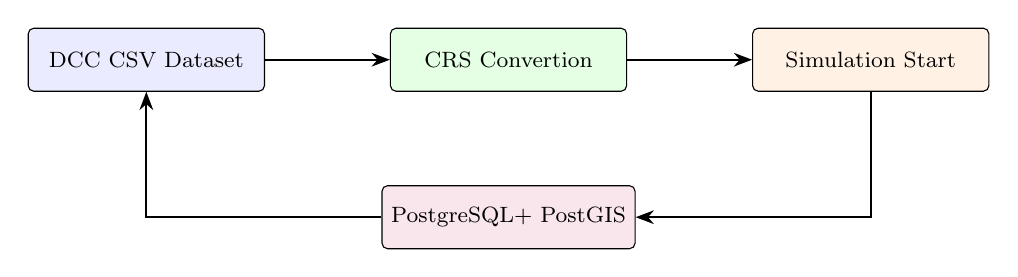
\begin{tikzpicture}[
  box/.style={rectangle, draw, rounded corners=2pt, fill=blue!8,
              minimum width=3.0cm, minimum height=0.8cm, text centered, font=\footnotesize},
  arrow/.style={-{Stealth}, thick}
]
\node[box] (csv) at (0,0) {DCC CSV Dataset};
\node[box, fill=green!10] (proj) at (4.6,0) {CRS Convertion};
\node[box, fill=orange!10] (init) at (9.2,0) {Simulation Start};
\node[box, fill=purple!10] (db) at (4.6,-2.0) {PostgreSQL\\+ PostGIS};
\draw[arrow] (csv) -- (proj);
\draw[arrow] (proj) -- (init);
\draw[arrow] (init) |- (db);
\draw[arrow] (db) -| (csv);
\end{tikzpicture}
\caption{Action Flow of the DCC public dataset implementation}
\label{fig:data_intake}
\end{figure}

\indent Like we showed in Fig~\ref{fig:data_intake} raw data processed for cordinate system with convertion to standart web mapping system WGS84 (EPSG:4326) it loaded into PostgreSQL database with enchanced spatial extension. This projects aims to use data driven techniques integration of IoT sensors and algorithmic optimization to show that we reduced the expenses of public garbage collection problem on bases of carbon emission and fuel cost.
\section{Problem Definition}

\indent In urban envoriments the garbage collection operations of the city suffers from two main problem like we mentioned before . The first problem is overflow risk that creates public health issues that problem can occur zones like Shopping Center,touristic attractions University Campuses and public transportation hubs.These heavy foot traffic areas has a faster ratio of fill level increase because of that natural habit of the zone the envorimental waste can create public health issues if we dont act before it occurs.


\indent Second inefficiency that we mentioned is lack of usage. That problem is a more complex and dangerous source of increasing cost.In fixed route systems trucks dispatches without looking at the fullness level of a bin and make a stop at those bins with half or lower fullness level.That means our trucks dispatch for a unnecesary low fullness level bins  and those inefficient dispatchs creates  significant cumulative waste of fuel and increasing amount of Carbon emission that can be preventable.


\indent Based on Eurostat statistics city waste management cover \%3--5 percent of the total cost of energy consumption ~\cite{eurostat2022}.A city like Dublin that has a population over a 1.4 million people that ratio ; translates to fuel,operational costs, and cost of the vehicle maintenance.The traditional systems cannot adjust their routes dynamically based on the bins fullness levels that is a well documented limitation that has driven research into IoT based monitoring and algorithmic route optimization solutions

\indent When we try to formalize this problem mathematically, it can be modelled as a dynamic version of a Capacitated Vehicle route problem (CVRP) with a time window. The main objective is to find a truck dispatch route that cover N containers, with a total cost (distance,fuel consumption,carbon emission) and reduce these fields to their lowest possible version of themselves.While doing that we should not allow any extra overflow in our system. Fig 1.2, shows us the fundamental difference between the fixed route approach and our dynamic route approach.

\begin{figure}[htbp]
\centering
\resizebox{\linewidth}{!}{%
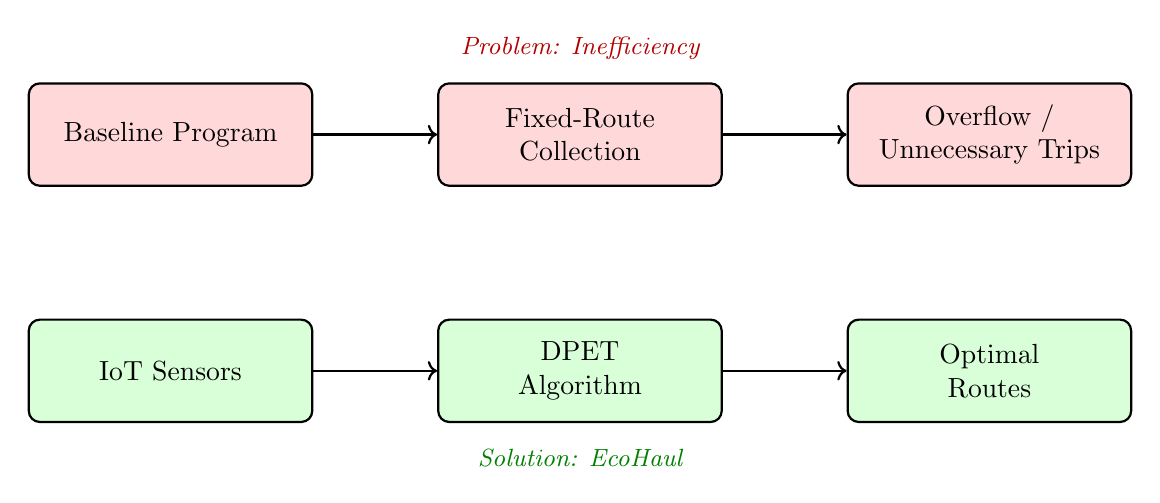
\begin{tikzpicture}[
    box/.style={
        rectangle,
        rounded corners,
        minimum width=3.6cm,
        minimum height=1.3cm,
        align=center,
        draw=black,
        thick
    },
    arrow/.style={
        ->,
        thick
    }
]

% Upper row (problem)
\node[box, fill=red!15]   (raw)    at (0,0)    {Baseline Program};
\node[box, fill=red!15]   (fixed)  at (5.2,0)  {Fixed-Route\\Collection};
\node[box, fill=red!15]   (waste)  at (10.4,0) {Overflow /\\Unnecessary Trips};

% Lower row (solution)
\node[box, fill=green!15] (sensor) at (0,-3)    {IoT Sensors};
\node[box, fill=green!15] (ml)     at (5.2,-3)  {DPET\\Algorithm};
\node[box, fill=green!15] (result) at (10.4,-3) {Optimal\\Routes};

% Titles
\node[font=\small\itshape, red!70!black] 
    at (5.2,1.1) {Problem: Inefficiency};

\node[font=\small\itshape, green!50!black] 
    at (5.2,-4.1) {Solution: EcoHaul};

% Arrows
\draw[arrow] (raw)    -- (fixed);
\draw[arrow] (fixed)  -- (waste);

\draw[arrow] (sensor) -- (ml);
\draw[arrow] (ml)     -- (result);

\end{tikzpicture}%
}

\caption{Overview of the problem and the proposed EcoHaul solution.}
\label{fig:problem_overview}
\end{figure}

\indent Fig~\ref{fig:problem_overview} upper part of the image represent the current state of the cities that uses fixed routes  predetermined dispatch programs inevitably ends up with extra unnecessary dispatchs or overflows because of the nature of this method.Lower part of the image represent our approach with data driven decision systems that got his data from real time sensor data that creates the ability of data driven efficient decision systems for garbage collection.Our optimized dispatch systems prevents the unnecesary dispatch routes for trucks and preventation of overflow that can cause public health issues

\section{Motivation}

\indent When we decide to develop ECO HAUL there were three key overlapping technological  and societal  trends.These three trends make our solution affordable and reachable for every city in the world 

\indent \textbf{First Motivation source is} affordable IoT Hardware getting more and more popular through time.Ultrasonic distance sensors getting combined with ESP32 microcontroller creates affordable components, that combination make city wise survey of fullness level more affordable and feasible. A couple dollar worth of Sensor device could get data necesarry data from a bin and with wifi it can transmit the data to headquarter.That was a capabilty that only expensive industrial systems can afford.

\indent \textbf{Second Motivation source is},Open source mapping and cloud computing device getting  more stable over a time.Tools like Leaflet and OpenStreetMap  allows us to develop scalable and affordable real time surveliance systems.Modern tools and libraries like FASTAPI,PostgreSQL and React allows us to develop systems to  process and visualize thousands of sensor data in real time with minimal delay.

\indent \textbf{Third Motivation source is} increasing amount of the sustainability goals of cities and European Union  climate goals.Cities are getting pressure on the matters like reducing their carbon foot print and cost of their public services.Optimizing the Waste management systems  can provide measurable  fuel and carbon emission savings.Because of the measurable savings smart waste management systems becomes a leverage in order to achieve these envorimental goals of the cities.

\indent Dublin City Council's public dataset creates a fundamental environment to combine these three motivation sources.The quality of the data we use comes from the 3,424 geographically referenced bin locations in Dublin City, which makes ECO HAUL a system that works on real-life cities instead of a toy dataset.Creating a simulation with real life data makes our algorithmic results applicable to real cities' waste management systems.

\indent  Fig~\ref{fig:feedback_loop},It illustrates the closed-loop system established by EcoHaul.In this loop sensor data feeds the fill prediction module,Feel prediction module is one of the constrains that we consider while DPET algorithm decide the optimal route for a truck waiting for a dispatch,visual dashboard visualize the route in real time and all the system feeds the database with all the events that occured in this closed loop.

\begin{figure}[H]
\centering
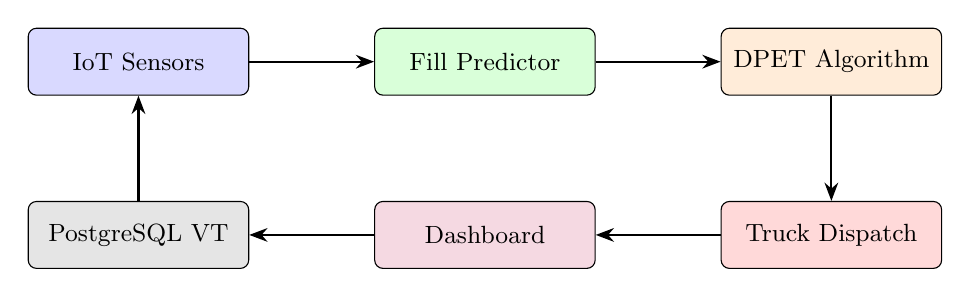
\begin{tikzpicture}[
  box/.style={rectangle, draw, rounded corners=3pt,
              minimum width=2.8cm, minimum height=0.85cm, text centered, font=\small},
  arrow/.style={-{Stealth}, thick}
]
\node[box, fill=blue!15]   (sensor)  at (0,0)     {IoT Sensors};
\node[box, fill=green!15]  (pred)    at (4.4,0)   {Fill Predictor};
\node[box, fill=orange!15] (dpet)    at (8.8,0)   {DPET Algorithm};
\node[box, fill=red!15]    (truck)   at (8.8,-2.2){Truck Dispatch};
\node[box, fill=purple!15] (dash)    at (4.4,-2.2){Dashboard};
\node[box, fill=gray!20]   (db)      at (0,-2.2)  {PostgreSQL VT};
\draw[arrow] (sensor) -- (pred);
\draw[arrow] (pred)   -- (dpet);
\draw[arrow] (dpet)   -- (truck);
\draw[arrow] (truck)  -- (dash);
\draw[arrow] (dash)   -- (db);
\draw[arrow] (db)     -- (sensor);
\end{tikzpicture}
\caption{Closed loop of the project EcoHaul .}
\label{fig:feedback_loop}
\end{figure}



\indent This feedback loop is important because we need our system to dynamicly change decision while city creates the data.Every dispatch event is a new data about the fill habit of a particular bin and those datas are useful to determine our prediction modules correctness rate.With this closed loop our systems educate itself about the habit of the cities that uses DPET algorithm over a time.We are expecting our systems to get better over a time period that provides valuable data for us.

\section{Report Structure}

\indent \textbf {CHAPTER 2 (Related works)} The remainder of this report is organized as follows:
In this part we are gonna mention about the academic works and industrial systems that we get inspired from ;IoT driven waste surveillance and garbage collection fill, prediction  and machine learning smart city simulation and digital twin and other related works discussed in details on this part of the 

\indent \textbf{CHAPTER 3 (Analysis and Design)},In this part our architecture and design going to be introduced.We use a multilayer architecture with stack structure,simulation engine,sequence diagram use case model, and database entity-relationship schema explained with details.


\indent \textbf{CHAPTER 4 (Application)}, In this part we show the details and development decisions on ECO HAUL's multi layer structure.Dual world simulation engine, DPET Dispatch algorithm with its six layer structure,Median filtering and ETF based Fill predictor,Urban environment Model , anomaly detection sub system,ESP32 IoT hardware layer,FastAPI backend and React frontend layer explained with important details.


\indent \textbf {CHAPTER 5 (Test and Results)},In this part we show our test cases that we do on system and achieve some quantitative evaluation results ; Our main concerns in this part is comparison of DPET with alternative strategy  KPI analysis , dispatch route efficiency , anomaly detection rate and system performance metrics.All the concerns and their measurements discussed in this part of the report.

\indent  \textbf{CHAPTER 6 (Future Work)}
In this part we discuss the future work and improvements that we need for getting a better version of our systems.We share our future ideas in this part.

\section{Requirements}

\indent Development process in the project ECO HAUL , depends on identifying both functional and nonfunctional  requirements.Functional requirements are the main objectives about what our system must do,Non functional requirements shows us how our system should operate while achieving those functional requirements.
\subsection{Functional Requirements}

\begin{itemize}[leftmargin=1.5cm]
  \item \textbf{FG-1: Real time bin surveillance.}
        \indent ECO HAUL system should create a real time surveillance system for all the bins in the area and follow their fullness level while saving the time series measurements into database.That job allows us to analysis the past events on the bin and creates the necesarry data that we are going to use at training our prediction model.
  \item \textbf{FG-2: Dynamic Dispatch.}
        \indent System should trigger the truck dispatch considering DPET algorithm fullness level ETF prediction engine and traffic state and create a smart decision to rather trigger or not triggering the truck dispatch
  \item \textbf{FG-3: Parallel Fixed Route Simulation.}
        \indent For performance comparison between the predetermined fixed route and our DPET algorithm we should simulate both scenario at the same time on simulation engine and show the differance between the KPI values.
  \item \textbf{FG-4: KPI Comparison.}
        \indent ECO HAUL project must show the comparison between the KPI's (fuel consumption,CO$_2$ emisson , total distance, operational costs) and display those data with special API endpoint
  \item \textbf{FG-5: Anomaly Detection.}
        \indent System must detect certain anomalies that we determined as a enum those are : UnAuthorized garbage collection,Sensor errors,Critical Fullness level , Anormal amount of increase on fulness level etc.
  \item \textbf{FG-6: KPI DASHBOARD.}
        The system should show us a web-based dashboard that includes a live map, color-coded container status, animated truck tracking system, and an KPI comparison panel.
  \item \textbf{FG-7: IoT Integration.}
        \indent While system using simulation engine and creates scenarios for our solution it also needs to accept data from ESP-32 and combined sensors and process those data with REST API endpoint.That makes our system syncronized  the ESP-32 and distance sensor data  with our software dependent simulation engine.
        
  \item \textbf{FG-8: Simulation Speed.}
        System must support an adjustable speed control for the simulation duration (i.e 1$\times$, 60$\times$, 3600$\times$, 86400$\times$).
\end{itemize}

\subsection{Non Functional Requirements}

\begin{itemize}[leftmargin=1.5cm]
  \item \textbf{FOG-1: Performans.}
        
        \indent API endpoints should respond under 200\,ms and can get atleast 50 simultanious Post request from differant sensors.
        \clearpage
  \item \textbf{FOG-2: Scalability.}
        System should support 3421 container without having a performance issue or a crash in a simulation.
  \item \textbf{FOG-3: Modularity.}
        \indent Simulation Engine , DPET algorithm, prediction engine , anomaly detection and API layer should significantly separetad from each other that makes things easier for future implementations and bug fixing.
 
\end{itemize}

% ===================== BÖLÜM 2 ==============================
\chapter{RELATED WORK}

\indent This section is for examining the academic research and industrial systems that inspire the development process of the project ECO HAUL.We examine those studies in four fundamental categories IoT driven waste surveillance ,Dynamic routing optimization for Garbage collection and truck dispatching,Fullness state prediction and approachs for prediction engine,Smart city simulation and digital twins.We mention about the categories and how they effect our project.
\section{IoT Driven Smart Waste Collection}

\indent The Application of IoT sensor on garbage collection surveillance is a trending research field since early 2010's.The main idea on this application is transmit fullness state data with  wifi connection to a headquarter.

\indent Gutierrez and his colleagues ~\cite{gutierrez2015}, advise us to use one of the early stage IoT driven Smart waste  management systems.In their works they use ultrasonic distance sensor with web based surveillance system.In this system they demonstrated if we use routing trucks for only a set of bins that exceed a certain fullness level dispatches we reduce the cost up to  \%40.The most important contribution of this study is it shows that we can use a basic HTTP based protocol to transmitt data.Project ECOHAUL inspired by this API design.Using physical ESP32 sensor data in our simulation engine with REST API endpoints is a natural extension of this idea.

\indent Arebey and his colleagues ~\cite{gutierrez2015} use a computer vision based approach on fullness level detection.From cameras that mounted on containers they take image data and with Gray Level Co-occurrence Matrix (GLCM).They process this images with feature extraction and predict the fullness level with this Gray Level Co-occurrence Matrix (GLCM) data.This approach proves that we can predict the fullness level with contactless  measurement without any mechanical level keys.Our project ECO HAUL prefers ultrasonic sensor for this contactless  measurement goal with more affordable method.


\indent Pardini and his colleagues ~\cite{pardini2018}, study provided a comprehensive literature review on IoT-based solid waste management solutions and showed that ESP32-class hardware, when combined with ultrasonic sensors, is feasible for long-term outdoor deployment. It particularly highlighted that low power consumption and durability are critical factors for the success of such systems. In response to these findings, EcoHaul’s ESP32 software incorporates design choices such as deep sleep mode and RTC memory persistence, which directly address these requirements.

\indent Bigbelly smart containers are working on commercial zone with solar energy, these containers can transmitt real time fullness data with wifi to a headquarter with compression mechanism.Datasets like DCC (Dublin City Council) includes bins like BigBelly smart bins means that smart waste managements systems are trending topic on real life city solutions.This example proves that modelled scenario for our project is realistic for real life usage.

\section{Vehicle Routing for garbage collection}

\indent Waste management problem is a variation of CVRP Capacitated Vehicle Route Problem variation a known NP-Hard problem ~\cite{dantzig1959}. Dantzig and Ramser's important study of truck dispatch problem.It define the problem for the first time and create a fundamental core for next studies on this field.NP-Hard problems by the nature cannot achieve the optimal solutions in reasonable time;thats why heuristic and metaheuristic approach is a necessity for the solution of this kinda problems.


\indent Christofide's algorithm ~\cite{christofides1976}, is a traditional method that guarantee $\frac{3}{2}$ ratio for Traveling Salesman Problem(TSP).This is one of the heuristic algorithm that worst case scenario of the algoritmh performance proven .It creates the foundation of the useage 2-opt at our RouteBuilder  theoratical layer.Classic approaches such as the Clarke–Wright savings algorithm and the nearest-neighbor heuristic have long been applied to municipal scheduling; EcoHaul uses the nearest-neighbor heuristic to generate an initial route and then optimizes it using the 2-opt algorithm.

\indent Akhtrar and his colleagues ~\cite{akhtar2017},They proposed a backtracking search optimization algorithm applied to CVRP for solid waste collection and, in particular, presented a
\textit{mass-dependent fuel consumption model}.In his studies he shows that considering mass while calculating the cost function is a important aspect of this problem.This information is a main source of motivation for the mass aware routing technique that we used on project ECO HAUL. We formulate the segment cost like this 

\begin{equation}
  C_{ij} = \bigl(m_{\text{baz}} + m_{\text{mevcut}}\bigr) \cdot d_{ij} + P_{\text{durak}}
  \label{eq:mass_aware}
\end{equation}

\indent In the figure $m_{\text{base}} = 12{.}000$~ kg is empty weight of the turck.$m_{\text{current}}$ represent the total weight that we got from the previous containers $d_{ij}$ represents the distance between the two stop point $P_{\text{Stop point}}$ represent the penalty of standing by while collecting garbage.This formulation based on Newton mechanics  $F = m \cdot a$ a heavier vehicle needs more force to save its acceleration . At standard CVRP  most of the heuristic only optimize the distance we run.Project ECOHAUL considers the total mass we carry between two stop that provides a more accurate cost model for real world application


\section{Fill Prediction}
\indent In reactive systems we take action only after a bin got into critical full state but in proactive system predicts the fill rate and take early action to prevent overflows.These proactive actions depends on prediction model like we used in project ECO HAUL

\indent Anagnostopoulos and his colleagues ~\cite{anagnostopoulos2015}, has proposed a queue-based dynamic container allocation framework that outperforms reactive systems by predicting demand clusters through spatial clustering. The most important finding of their work is that containers located within the same geographic cluster exhibit similar filling rate characteristics driven by common environmental factors. For example, all containers in a shopping district exhibit similar hourly filling patterns. This finding directly motivated the K-means region assignment in project EcoHaul  filling predictor; the system clusters 3,424 containers into 12 geographic regions to provide more reliable predictions at the regional level.



\indent Malapur and Pattanshetti ~\cite{malapur2017}, uses a gradient boosted trees that been trained by a fill data for proactive dispatch.Their study shows that machine learning has outperforms traditional threshold-based methods in occupancy prediction.This approach requires to periodicly trained data for batching process.Project ECO HAUL choose a more feasible solution for real time simulation we look at the logs of the past events that happened before  and use those events in a sliding time window approach that creates a prediction module that doesnt required to constant train to be able to process.

\section{Smart City Simulation and Digital Twin}


\indent Parallel world simulations  in the Project ECO HAUL is strongly related with digital twin approach.Digital Twin is a copy of a physical system in real life to create what-if scenarios on those real life aspect. 


\indent Grieves ve Vickers~\cite{grieves2017} release the pioneering study of digital twin concept into academical litreture.In their idea of digital twin get together on a physical existence and a digital existence in between these existences we transmitt data.Later studies use that approach to examine the urban infrastructure monitoring.Project ECO HAUL is a digital twin for a Dublin garbage collection network.Creates a solid foundation for a methodological compare between a fixed route and DPET algorithm with his parallel simulation approach creates a controlled experiment envoriment for impossible real life scenarios.

\indent Anagnostopoulos and his colleagues  ~\cite{zanella2014} shows us a fundamental IoT architecture for  Smart Cities.Their study  ; communication protocols , data models and has defined interoperability requirements in detail.They effect the combined machine API structer of project ECO HAUL; both physical ESP32 sensors and software simulation engine  connected to  a single REST interface that operates without any changes. This unified approach enables the system to be gradually expanded with actual hardware.


\begin{figure}[H]
\centering
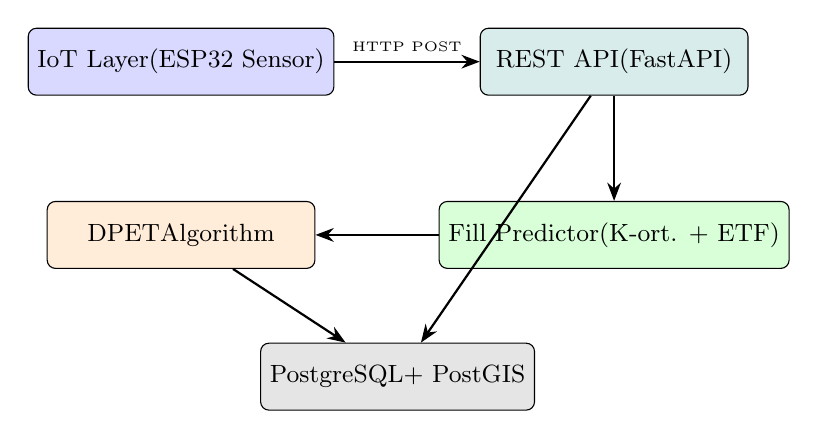
\begin{tikzpicture}[
  box/.style={rectangle, draw, rounded corners=3pt,
              minimum width=3.4cm, minimum height=0.85cm, text centered, font=\small},
  arrow/.style={-{Stealth}, thick}
]
\node[box, fill=blue!15]   (iot)   at (0,0)     {IoT Layer\\(ESP32 Sensor)};
\node[box, fill=teal!15]   (api)   at (5.5,0)   {REST API\\(FastAPI)};
\node[box, fill=green!15]  (ml)    at (5.5,-2.2){Fill Predictor\\(K-ort. + ETF)};
\node[box, fill=orange!15] (dpet)  at (0,-2.2)  {DPET\\ Algorithm};
\node[box, fill=gray!20]   (db)    at (2.75,-4) {PostgreSQL\\+ PostGIS};
\draw[arrow] (iot)  -- node[above,font=\tiny]{HTTP POST} (api);
\draw[arrow] (api)  -- (ml);
\draw[arrow] (ml)   -- (dpet);
\draw[arrow] (dpet) -- (db);
\draw[arrow] (api)  -- (db);
\end{tikzpicture}
\caption{EcoHaul System Component Interaction Diagram.}
\label{fig:component_interaction}
\end{figure}


\Fig~\ref{fig:component_interaction} below shows us the mentioned methods and how their getting together in our Project ECOHAUL architecture.The data comes from IoT layer goes to a RESTAPI endpoint and trigger the prediction module with DPET algorithm,results are getting permanent in a PostgreSQL database.
% ===================== BÖLÜM 3 ==============================
\chapter{ANALYSIS AND DESIGN}

\indent This section is a  detailed explaination of the architectural structure of project ECOHAUL.Firstly  we explain the multilayer architecture of the project then we continue with the logical explanation of how we use the simulation engine on our project;Next, the component interactions in a shipment cycle are addressed using a sequence diagram, the system functions using a use-case diagram, and the data organization using an entity-relationship diagram. EcoHaul system component interaction diagram.Project ECOHAUL designed as a full stack application that make data driven decision and real time visualization.

\section{Dataset Definition}


\indent The main dataset of the project comes from Dublin City Council public data center's garbage bin location dataset.This dataset provides  us the geographical location of the bin's and their cordinates city wise also their kind and city zone information inclued in this data set our Table ~\ref{tab:dataset} sum up all the important features of this main dataset.

\begin{table}[H]
\centering
\caption{Dublin Belediyesi kamusal konteyner veri seti özellikleri.}
\label{tab:dataset}
\begin{tabular}{ll}
\toprule
\textbf{Feature} & \textbf{Value} \\
\midrule
Total records        & 3,424 waste containers \\
Original CRS         & Irish Transverse Mercator (EPSG:2157) \\
Web CRS              & WGS84 (EPSG:4326) \\
Geographical coverage & Dublin city center and surrounding areas \\
Approximate center   & 53.34$^\circ$N, 6.27$^\circ$W \\
Container types      & Cast Iron, Bigbelly Solar, Class A/B, Dog Waste \\
Data format          & CSV (x/y coordinates, type, region) \\
\bottomrule
\end{tabular}
\end{table}


\indent The bins in the dataset has differant features. \textit{Cast Iron} bins is the traditional garbage bins on the city. \textit{Bigbelly Solar} bins are the new technology bins that uses solar power with a press machine in their space those bins also can report their fullness level in real life so that approves ECO HAUL's sensor based approach is a proven approach in real life . Having this many differant type of bins in our dataset represent the real life  diversity.


\indent Raw dataset has only the information about geographical cordinates thats why we need a simulation engine that creates a generic real life data at the begining.This simulation engine is not working randomly the data that we produce depends on many things such as geographical zone type and statistically weighted distributions. Tablo~\ref{tab:bin_attrs}, Shows us the starting features for the bins that we genericly create.

\begin{table}[H]
\centering
\caption{Synthetic attributes assigned to containers at the start of the simulation.}
\label{tab:bin_attrs}
\begin{tabular}{llll}
\toprule
\textbf{Attribute} & \textbf{Value} & \textbf{Filling Rate} & \textbf{Assignment Basis} \\
\midrule
filling\_label A & High traffic   & 12--16 \%/hr   & Weighted random selection \\
filling\_label B & Medium traffic & 4--8 \%/hr     & Weighted random selection \\
filling\_label C & Low traffic    & 0.5--1.5 \%/hr & Weighted random selection \\
region\_type     & RESIDENTIAL    & Variable       & Region sequence matching \\
region\_type     & OFFICE         & Variable       & Region sequence matching \\
region\_type     & RETAIL         & Variable       & Region sequence matching \\
region\_type     & UNIVERSITY     & Variable       & Region sequence matching \\
region\_type     & TOURIST        & Variable       & Region sequence matching \\
\bottomrule
\end{tabular}
\end{table}

\indent Like we see in the table the fullness labels separate into three differant class: Containers with Label A increase their fullness level up to \%12--16  in an hour that makes them a heavy traffic area for garbage collection routes.Containers with Label B increase their fullness level up to \%4--8 mid  that makes them a mid-level traffic area for our dispatch algorithm.Containers with Label C increase their fullness level up to \%0.,5--1,5 mid  that makes them a low-level traffic area for our dispatch algorithm.This classification simulates the heterogeneous fill pattern in a real-life scenario for a crowded city.Zone types determined by string matching in a real world scenario DCC dataset provides these strings to us with a combination of our string and the labels that we determined gives us the profile of  a bin that we are going to use in our simulation.

\section{System Architecture}


\indent ECOHAUL builed on a significantly separate multi layer architecture.We showed the layers in  Fig~\ref{fig:arch_layers}
Like we see in the figure the layers are Database at the bottom,algorithm layer,simulation engine,REST API and at the top Visualization Dashboard.This multilayer structure allow us the achieve our goal to maintain a modular system with multi independent layer our development process and debugging sessions are relativly easy and feasible.

\begin{figure}[H]
\centering
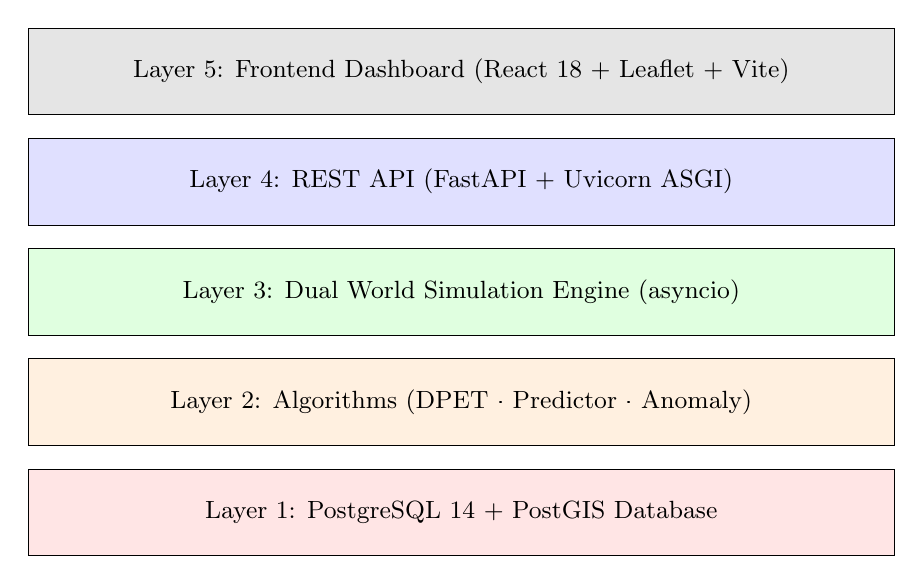
\begin{tikzpicture}[
  layer/.style={rectangle, draw, minimum width=11cm, minimum height=1.1cm,
                text centered, font=\small}
]
\node[layer, fill=gray!20]    at (0,5.2)  {Layer 5: Frontend Dashboard (React 18 + Leaflet + Vite)};
\node[layer, fill=blue!12]    at (0,3.8)  {Layer 4: REST API (FastAPI + Uvicorn ASGI)};
\node[layer, fill=green!12]   at (0,2.4)  {Layer 3: Dual World Simulation Engine (asyncio)};
\node[layer, fill=orange!12]  at (0,1.0)  {Layer 2: Algorithms (DPET \textperiodcentered\ Predictor \textperiodcentered\ Anomaly)};
\node[layer, fill=red!10]     at (0,-0.4) {Layer 1: PostgreSQL 14 + PostGIS Database};
\end{tikzpicture}
\caption{Multilayer Structure of EcoHaul .}
\label{fig:arch_layers}
\end{figure}


\indent \textbf{Layer 1 {Database}},stores the system's entire state on PostgreSQL, enhanced with the PostGIS spatial extension.Container telemetries stored in a PostGIS Point type ; that storage decision allow us to make queries like 'bins that 100 meters away from a specific truck' efficiently.


\indent \textbf{Layer 2 (Algorithms)},this layer contains the mind of the system:DPET dispatch algorithm , Median Filtering, ETF driven fill prediction and anomaly detection servis.This layer contains pure algorithmic logic and can be tested independently  from simulation engine layer.That allow us to try new approachs without crushing the entire system.


\indent \textbf{Layer 3 (Simulation Engine)},This engine working on a constant event loop while using a python library called \texttt{asyncio}.Two parallel world situation runs simultaniously the world that runs the DPET algorithm and the world that runs the fixed route algorithm that uses the predetermined TSP solution at 06:00 everyday works simultaniously in our dashboard.These two word shares the same container data and fill rate data to that makes the conditions of the both words identical the only differance between these words are their approach to the problem one of them uses a fixed route and our solution uses an algorithm called DPET.That structure is a fundamental design decision that allow us to achieve our goal at FG-3.



\indent \textbf{Layer 4 (REST API)}, That layer was builded on a FastAPI and Uvicorn ASGI server.In this layer we make our frontend to be able to communicate with our simulation engine and also with our physical ESP32 devices that grant us the fullness level data that ve achieve from real world.With this structure we obtain a combined KPI Dashboard



\indent \textbf{Layer 5 (Frontend)},This layer shows real time KPI dashboard with React and Leaflet.In this dashboard we obtain informations like CO$_2$ emission,total distance covered , fuel cost , efficiency that calculated by a special formula and also we can start our simulation engine open the anomaly page and decide the speed of our simulation.

\section{Flow Diagram}


\indent Once the system’s layered structure and overall data flow have been defined, it is important to specify the exact order in which these components communicate with eachother in practice.Fig~\ref{fig:sequence} allow us to see a typical garbage truck dispatch loop,with this diagram we are able to see how each component interact with each other in which order.

\begin{figure}[H]
\centering
\small
\begin{tikzpicture}[
  scale=1.25,
  transform shape,
  life/.style={draw, minimum width=1.6cm, minimum height=0.55cm,
               text centered, font=\tiny, fill=white},
  msg/.style={-{Stealth}, thin}
]

\foreach \x/\lbl in {0/Front-End, 2.8/FastAPI, 5.6/Sim Engine, 8.4/DPET, 11.2/PostgreSQL}{
  \node[life] at (\x, 0) {\lbl};
  \draw[dashed] (\x,-0.3) -- (\x,-9);
}

\draw[msg] (0,-0.8) -- node[above,font=\tiny]{GET /live-state}   (2.8,-0.8);
\draw[msg] (2.8,-1.3) -- node[above,font=\tiny]{get\_snapshot()}  (5.6,-1.3);
\draw[msg] (5.6,-1.8) -- node[above,font=\tiny]{SELECT bins}      (11.2,-1.8);
\draw[msg] (11.2,-2.3) -- node[above,font=\tiny]{bin states}   (5.6,-2.3);
\draw[msg] (5.6,-2.8) -- node[above,font=\tiny]{snapshot}         (2.8,-2.8);
\draw[msg] (2.8,-3.3) -- node[above,font=\tiny]{JSON 200}         (0,-3.3);

\draw[msg] (5.6,-4.2) to[loop right]
node[right,font=\tiny]{Fill level Update} (5.6,-4.2);

\draw[msg] (5.6,-5.2) -- node[above,font=\tiny]{trigger\_dispatch(bins)} (8.4,-5.2);

\draw[msg] (8.4,-5.7) to[loop right]
node[right,font=\tiny]{Bin Scoring \& Picking} (8.4,-5.7);

\draw[msg] (8.4,-6.4) to[loop right]
node[right,font=\tiny]{Build Route (NN+2-opt)} (8.4,-6.4);

\draw[msg] (8.4,-7.1) -- node[above,font=\tiny]{Dispatch plan}   (5.6,-7.1);

\draw[msg] (5.6,-7.8) -- node[above,font=\tiny]{INSERT events}   (11.2,-7.8);

\draw[msg] (11.2,-8.3) -- node[above,font=\tiny]{commit OK}       (5.6,-8.3);

\end{tikzpicture}
\caption{Sequence Diagram of the EcoHaul Simulation Dispatch Cycle.}
\label{fig:sequence}
\end{figure}
\subsection{Flow Definition}

\indent Flow in the diagram starts with frontend sending \texttt{GET /live-state} request at regular intervals.Fast API pass this request to simulation engine;engine triggers \texttt{get\_snapshot()} function and create a query for PostgreSQL to take container state datas and return a snapshot that include all the current states of garbage collection trucks and garbage collection containers.That snapshot converted into JSON format and forward to the frontend with this data frontend create a real time visualization of the current state.This loops triggers everysecond until the simulation ends

\indent Simulation engine inner clock continues simultaniously to that query loop.With each tick three major job triggers : First of all \textbf{fill job} triggers this job controls the fill level increases for every container in the simulation that fill job updates depends on the simulation models that creates labels and special zones.The system continues with \textbf{Anomaly job} this job triggers random anomalies in the simulation for example sensor errors , unusual fill speed , unauthorized hauling  and overflow risks.This job also controls the anomalies that happened both in the simulation and real word data that comes from ESP32.

\indent When the dispatch interval is triggered (every simulation hour in the DPET world), the engine initiates the DPET algorithm with the current container state list via the trigger dispatch call. DPET processes the containers through its six-layer pipeline: first scoring and selecting, then constructing the route using nearest neighbor and 2-opt. The algorithm returns a completed dispatch plan to the simulation engine. The engine creates simulated truck objects based on this plan; as the trucks follow the route, it records collection events and truck telemetry in the database using \texttt{INSERT} queries. When the database returns a commit OK, the loop completes and waits for the next tick.

\section{Use Case Diagram}

\indent Before we explain the functionalities in detail we create a use case diagram to show this functions and how they are interaction with different actors in our system. Fig~\ref{fig:usecase} is the answer of  'what ECOHAUL do' for different actors that have a part in this system

\begin{figure}[H]
\centering

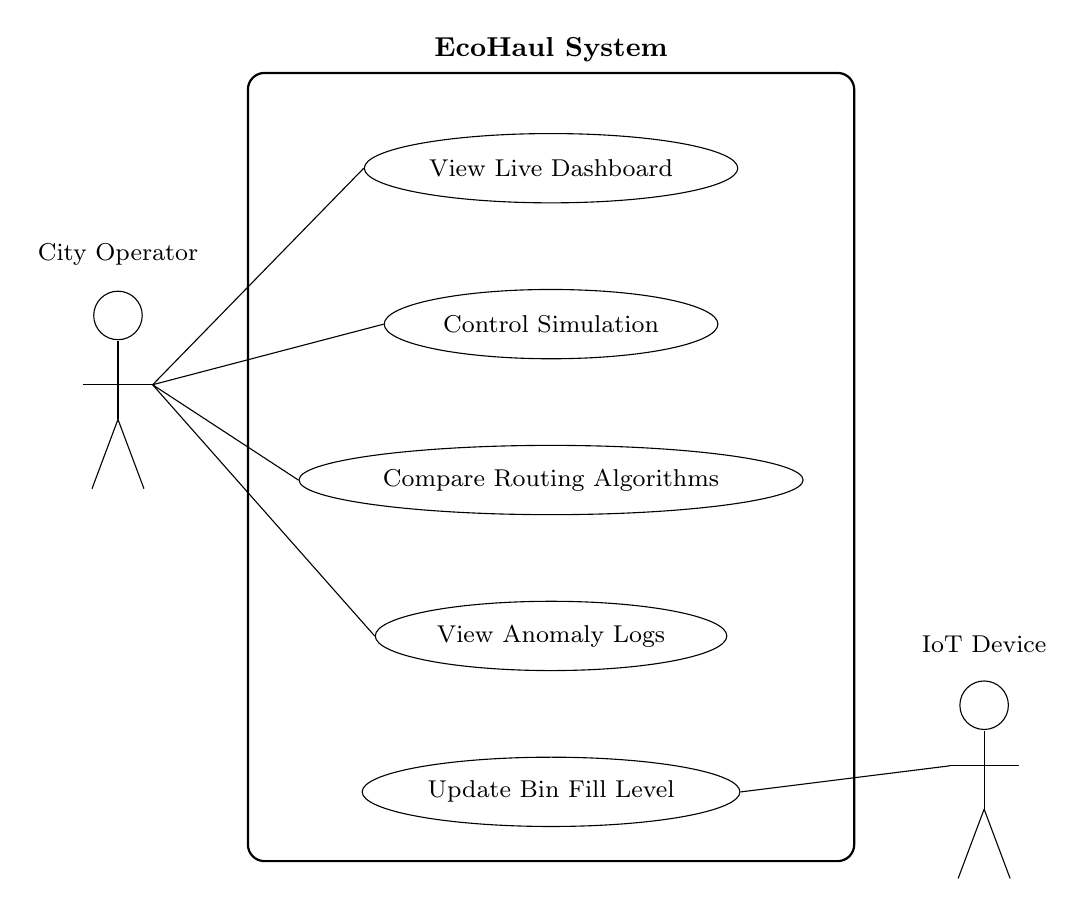
\begin{tikzpicture}[
    scale=1.1, 
    transform shape,
    font=\small
]

% System Boundary - Alt sınır -9.5'e çekilerek uzatıldı
\draw[thick, rounded corners=6pt] (1.5,-0.4) rectangle (8.5,-9.5);
\node[above, font=\small\bfseries] at (5.0,-0.4) {EcoHaul System};

% City Operator Actor - Konumu orta noktaya göre ayarlandı
\node[font=\footnotesize] at (0,-2.5) {City Operator};
\draw (0,-3.2) circle (0.28cm);
\draw (0,-3.5) -- (0,-4.4);
\draw (-0.4,-4.0) -- (0.4,-4.0);
\draw (0,-4.4) -- (-0.3,-5.2);
\draw (0,-4.4) -- (0.3,-5.2);

% IoT Device Actor - Konumu en alttaki use case'e göre ayarlandı
\node[font=\footnotesize] at (10,-7.0) {IoT Device};
\draw (10,-7.7) circle (0.28cm);
\draw (10,-8.0) -- (10,-8.9);
\draw (9.6,-8.4) -- (10.4,-8.4);
\draw (10,-8.9) -- (9.7,-9.7);
\draw (10,-8.9) -- (10.3,-9.7);

% Use Cases - Aralarındaki mesafe (y ekseni) 1.3'ten 1.8'e çıkarıldı
\node[
draw,
ellipse,
minimum width=3.8cm,
minimum height=0.8cm,
font=\footnotesize
] (uc1) at (5.0,-1.5) {View Live Dashboard};

\node[
draw,
ellipse,
minimum width=3.8cm,
minimum height=0.8cm,
font=\footnotesize
] (uc2) at (5.0,-3.3) {Control Simulation};

\node[
draw,
ellipse,
minimum width=3.8cm,
minimum height=0.8cm,
font=\footnotesize
] (uc3) at (5.0,-5.1) {Compare Routing Algorithms};

\node[
draw,
ellipse,
minimum width=3.8cm,
minimum height=0.8cm,
font=\footnotesize
] (uc4) at (5.0,-6.9) {View Anomaly Logs};

\node[
draw,
ellipse,
minimum width=3.8cm,
minimum height=0.8cm,
font=\footnotesize
] (uc5) at (5.0,-8.7) {Update Bin Fill Level};

% Associations - Aktör kollarından use case'lere bağlantılar
\draw (0.4,-4.0) -- (uc1.west);
\draw (0.4,-4.0) -- (uc2.west);
\draw (0.4,-4.0) -- (uc3.west);
\draw (0.4,-4.0) -- (uc4.west);

\draw (9.6,-8.4) -- (uc5.east);

\end{tikzpicture}

\caption{Use case diagram of the EcoHaul system .}
\label{fig:usecase}
\end{figure}


\indent In this diagram there are two main actor that effect the ECOHAUL system. First actor is City Operator this actor is a human that uses our system.It triggers the fundamental features of the system : live dashboard view, simulation start/pause/speedup control.KPI comparison of the two parallel world (DPET and fixed route),inspect the view of the occured anomalies and so on. Second actor is \textbf{IoT Device (ESP32 sensor)} this actor autonomiously checks the fullness data  and triggers end points for jobs like update container fullness level and state . This dual actor structure demonstrates that project ECOHAUL can work with both human-monitored and automated data sources.

\section{Entity-Relationship Diagram}

\indent In this section we look into the organization of data that we store in our database and their relationship with entities.Data models  was designed in accordance with normalization principles to ensure data integrity and prevent unnecessary data duplication in our dataset.ECOHAUL dataset  has been implemented on PostgreSQL using the PostGIS spatial extension.Table ~\ref{tab:db_tables} defines the five fundamental table and their purpose in the system

\begin{table}[H]
\centering
\caption{Database table definitions.}
\label{tab:db_tables}
\begin{tabular}{llp{6.8cm}}
\toprule
\textbf{Table} & \textbf{Primary Key} & \textbf{Purpose} \\
\midrule
bins              & id (VARCHAR)  & Static bin metadata, current fill level, PostGIS POINT geometry, region, and active flag \\
telemetry         & id (SERIAL)   & Time-series fill measurements (Foreign Key: bin\_id) \\
event\_log        & id (SERIAL)   & Anomaly, dispatch, and heartbeat events; flexible JSONB detail field \\
truck\_telemetry  & id (SERIAL)   & Simulated truck GPS traces during active routes \\
collection\_events & id (SERIAL)  & Bin emptying records with timestamp and truck ID \\
\bottomrule
\end{tabular}
\end{table}

\indent \texttt{bins} table is fundemantel asset to our system; all the other tables apply to that bin table with foreign keys.This table holds the static meta data (id, type, zone) , current fullness state and PostGIS POINT geometry datas.\texttt{telemetry} table stores all the bin fullness measurements in a time series and those data are mainly used on prediction model training.



\indent The \texttt{event\_log} table is particularly noteworthy in our architecture, as it incorporates a \texttt{JSONB} detail column to handle diverse metadata requirements. That design choice provides the flexible storage of event-specific data—such as truck proximity during unauthorized emptying events or the discrepancy between expected and actual fill levels in skip anomalies—without the need for constant schema updates. By leveraging this approach, we ensure that the system remains highly extensible; new anomaly types can be integrated easily without altering the underlying database structure, thereby ECOHAUL's is higly flexiable to extensions when needed. 
% ===================== BÖLÜM 4 ==============================
\chapter{IMPLEMENTATION}

\indent In this section we explain the main components like simulation engine , DPET dispatch algorithm,fill predictor,urban envoriment model,anomaly detection system,ESP32 IoT Layer , FastAPI front end and backend with implementation details.Every component  introduced with their basic logical explanation.

\section{Simulation Engine}

\indent Simulation engine (\texttt{simulation\_engine.py}, $\approx$800 line) is the main component of the system.This component uses the python library called   \texttt{asyncio}  to build a modular and extendable while build a two world simulation.Two independent  \texttt{WorldState}  object simulates simultaniously  one of them is DPET world and the other world represent the fixed route world.Simulation engine runs with seperate ticks and every tick triggers three job

\begin{enumerate}[leftmargin=2cm]
   \item \textbf{Fill Job} --- Engine updates the fill level according to current urban envoriment model.This process applies multipliers based on region type, time zone, and active events
  \item \textbf{Anomaly Job} --- Controls every single container for anomali states such as , sensor errors , overflow risks, unauthorized hauling and etc.After this control it saves the detected anomalies into \texttt{event\_log} table.
  \item \textbf{Dispatch Job} --- In this job we evaluate the dispatch triggers for both of the world.In the world that we used DPET algorithm we trigger the six layer algoritm work,in the predetermined world we check whether the time is 06:00 clock or not.
\end{enumerate}

\indent Listing~\ref{lst:tick},Show us the basic loop of the simplified tick loop structure. The loop measures the elapsed real time at each tick and advances the simulation time based on the speed factor.

\begin{lstlisting}[language=Python, caption=Simplified simulation tick loop structure., label=lst:tick]
async def _tick_loop(self):
    while self._running:
        tick_start = time.monotonic()
        sim_dt = TICK_S * self._speed_mult
        self._sim_time += sim_dt

        await self._run_fill_job()       # all bin fullness update
        await self._run_anomaly_job()    # anomaly detection
        await self._run_dispatch_job()   # Dpet and fixed route trigger

        elapsed = time.monotonic() - tick_start
        await asyncio.sleep(max(0.0, TICK_S - elapsed))
\end{lstlisting}
\indent Speed multiplier architecture is the most significant experimental feature of the system this system design allow us to meet the needs of FG-8 Adjustable Simulation Speed.On 3600$\times$ in this speed one simulation hour equals to one second in real time that means a 30 day simulation interval approximetly 40 real life minute.This allows for a comprehensive algorithmic evaluation without waiting for real-time completion. The speed factor can be adjusted at runtime; for example, an operator can reduce speed to 1$\times$ for monitoring an interesting event in detail.

\section{DPET Algorithm}

\indent Dpet Algorithm (\texttt{dpet.py}, $\approx$450 line),this module create a convertion job with its six layer pipeline it converts current container states into optimized dispatch plan.These six layer includes all the decision process from raw fullness data to routes that we used for optimization world.
\clearpage
\subsection{Layer 1: Traffic Model}
\indent The first layer assigns a time-dependent traffic score $T \in [0, 1]$ to each simulation hour. Peak hours (07:00-–09:00 and 17:00–-19:00) receive $T = 0.80$; off-peak hours receive $T = 0.50$; and quiet hours receive $T = 0.20$. A container is marked as \textit{traffic-friendly} when $T < 0.6$. This layer ensures that non-critical pickups are rescheduled to off-peak hours to prevent trucks from getting stuck in heavy traffic and wasting fuel.


\subsection{Layer 2: Container Evaluater}

\indent The second layer assigns a composite priority score $S$ to each active container, consisting of five weighted components:

\begin{equation}
  S = 0{,}40\,s_{\text{fullness}} + 0{,}35\,s_{\text{ETF}} + 0{,}12\,s_{\text{traffic}} + 0{,}08\,s_{\text{density}} + 0{,}05\,s_{\text{distance}}
  \label{eq:bin_score}
\end{equation}
\indent The choice of the five weights is grounded in the operational
objectives encoded in the algorithm. The two dominant components---fullness
($0{,}40$) and ETF ($0{,}35$)---together carry $75\%$ of the score because they
are the only two signals that directly measure overflow risk: $s_{\text{fullness}}$
captures the \textit{current} state of a container, while $s_{\text{ETF}}$
captures its \textit{predicted} future state. Fullness is given the single
largest weight because an already-full bin is a certainty, whereas ETF is a
forecast and is therefore weighted slightly lower to account for prediction
uncertainty; nonetheless ETF is kept close to fullness so that the system can
act \textit{before} an overflow rather than only reacting to one. The remaining
three weights are deliberately small ($0{,}12 + 0{,}08 + 0{,}05 = 0{,}25$): traffic,
density and proximity are cost-efficiency refinements, and they are bounded so
that they can re-order containers of \textit{similar} urgency but can never
promote an empty bin above a near-full one. Among these, traffic receives the
largest share ($0{,}12$) because it has the greatest impact on travel time and
fuel during rush hours, density follows ($0{,}08$) as it enables servicing a
cluster of bins in a single trip, and proximity is smallest ($0{,}05$) because
depot distance only affects the initial dead-mileage of a route. This ordering
($w_{\text{fill}} > w_{\text{ETF}} \gg w_{\text{traffic}} > w_{\text{density}} >
w_{\text{proximity}}$) directly encodes the design priority of the system:
overflow prevention first, operational cost second.

\indent It should be noted that the fullness component is not used linearly.
In the implementation the score is computed as $s_{\text{fullness}} =
(f/100)^2$, and for bins above $85\%$ an additional boost term pushes the score
further towards 1. This quadratic shaping ensures that the difference between a
$60\%$ and a $95\%$ bin is amplified, so that critically full containers
dominate the ranking even more strongly than their raw weight of $0{,}40$ would
suggest. Likewise, the ETF urgency is normalized over a $24$-hour horizon
($s_{\text{ETF}} = \max(0,\,1 - \text{ETF}/24)$), meaning that any container
predicted to overflow within the next day contributes a non-zero urgency
signal, with the contribution rising sharply as the predicted overflow time
approaches zero.

\subsection{Layer 3: Container Picker}

The first layer assigns a time-dependent traffic score $T \in [0, 1]$ to each simulation hour. Peak hours (07:00--09:00 and 17:00--19:00) receive $T = 0.80$; off-peak hours receive $T = 0.50$; and quiet hours receive $T = 0.20$. A container is marked as \textit{traffic-friendly} when $T < 0.6$. This layer ensures that non-critical pickups are rescheduled to off-peak hours to prevent trucks from getting stuck in heavy traffic and wasting fuel.

\indent This layered structure allows the system to prioritize emergencies while also opportunistically collecting data during periods of lower traffic volume.

\subsection{Layer 4: Route Builder}

\indent The fourth layer constructs an optimized route for the selected containers in three sub-steps:
\begin{enumerate}[leftmargin=2cm]
  \item \textbf{Nearest Neighbor Start} --- creates an initial route starting from the depot using the greedy nearest-neighbor heuristic.
  \item \textbf{Capacity Pruning} --- removes containers that would exceed the truck’s volume capacity (maximum of 40 stops per truck).
  \item \textbf{2-opt Improvement} --- Iteratively reverses the route’s sub-segments to minimize the mass-aware total cost defined in Equation~\ref{eq:mass_aware}.
\end{enumerate}

\indent The mass-aware cost function takes into account the weight of waste accumulated along the route. This reflects the physical principle $F = m \cdot a$: as the truck fills up, it becomes heavier and requires more fuel to maintain the same driving profile. Therefore, the algorithm attempts to find a sequence of stops that ensures heavy loads are transported over the shortest possible distances.

\subsection{Layer 5: Route Efficiency Filter}

\indent The fifth layer checks whether a route is viable for shipment.
The efficiency metric is defined as the ratio of the number of containers
collected along the route to the total distance travelled:
\begin{equation}
  \eta = \frac{N_{\text{container}}}{D_{\text{total}}} \geq 0.20 \;\text{container/km}
  \label{eq:efficiency}
\end{equation}

\indent Here $N_{\text{container}}$ is the number of stops on the route, and
$D_{\text{total}}$ is the complete round-trip distance, measured from the depot
to the first stop, through all intermediate stops, and back to the depot


\indent The threshold value of $0.20$ container/km is equivalent to requiring,
on average, at least one container collected per five kilometres travelled
($1/0.20 = 5\,\text{km}$). Routes that fall below this value are rejected,
because they would dispatch a truck to collect only one or two containers over
a long distance, wasting fuel and vehicle time. This filter therefore acts as a
critical checkpoint that prevents economically and environmentally inefficient
trips.


\indent The filter is not applied unconditionally. If a route contains at least
one urgent container---one whose fill level has reached the emergency threshold
or whose estimated time-to-full has dropped below the dispatch lead time---the
efficiency check is bypassed and the route is approved regardless of its
$\eta$ value. This guarantees that overflow-critical containers are always
serviced, even when doing so is not strictly efficient.

\subsection{Layer 6: Dispatcher}

\indent The sixth and final layer determines the number of trucks required to cover the selected containers (each truck can handle up to 40 stops) and creates the simulated truck objects. The maximum fleet size is limited to 12 trucks per world to reflect realistic municipal fleet constraints. The dispatcher hands off the generated trucks to the simulation engine; the engine moves these trucks along their routes and records the pickup events.

\section{Fill Level Predictor}

\indent The fill predictor (\texttt{predictor.py}, ≈300 lines) uses two mechanisms: spatial region assignment via K-means clustering and online TDZ learning from observed fill cycles. Together, these two mechanisms enable the system to make proactive dispatch decisions.

\subsection{K-Means Cluster Assignment}

\indent When the system is initialized, the coordinates of all 3,424 containers are clustered into $K = 12$ geographic regions using K-means++ followed by a Lloyd’s iteration. K-means++ reduces the risk of the standard K-means method getting stuck in a local minimum by intelligently selecting the initial centers. Containers located in the same region tend to share similar environmental characteristics; for example, all containers in a shopping district cluster together. This enables more reliable predictions at the regional level rather than relying on individual container predictions with limited historical data.

\subsection{ETF Training }

\indent Her The container estimator maintains a sliding window consisting of up to eight fill cycle durations. A cycle is defined as the time elapsed between two consecutive \texttt{EMPTIED} (emptied) events. The estimated fill rate is calculated as follows:

\begin{equation}
  \hat{r} = \frac{\%100}{\bar{T}_{\text{cycle}} / 3600}\;\; [\%/\text{hour}]
  \label{eq:fill_rate}
\end{equation}

\indent and the Estimated Time to Fill (ETF) is calculated as follows:

\begin{equation}
  \text{ETF} = \frac{\%100 - f_{\text{current}}}{\hat{r}}\;\; [\text{hour}]
  \label{eq:etf}
\end{equation}

\indent In these formulas, $\bar{T}_{\text{cycle}}$ represents the average cycle time (in seconds), and $f_{\text{current}}$ represents the container’s current fill percentage. The moving window approach allows the system to place greater weight on recent observations and adapt to changing conditions. When the ETF value of at least 6 containers in the same region falls below the forecast horizon $H_{\text{forecast}} = 7$ hours, a proactive shipment is triggered for that region; this is a key parameter that balances proactive collection with route density requirements.

\section{Urban Envoriment Model}

\indent The Urban Environment Model (\texttt{environment.py}, ≈280 lines) modulates waste generation rates using area-specific hourly profiles and random urban events. This model is a critical component that enables the simulation to reflect the complex and variable waste generation patterns of a real city. Five area archetypes are modeled:

\begin{itemize}[leftmargin=1.5cm]
  \item \textbf{RESIDENTIAL}: Waste generation typically peaks between 18:00 and 20:00 at around 1.7--2.0$\times$ the normal level, while nighttime activity remains relatively quiet. This pattern reflects people returning home after work.
  
  \item \textbf{OFFICE}: Activity usually reaches its peak between 08:00 and 10:00 at approximately 0.9--1.9$\times$ the baseline level and becomes significantly quieter after 20:00, following standard working hours.
  
  \item \textbf{SHOPPING}: Waste levels increase noticeably between 15:00 and 20:00, reaching around 1.9--2.4$\times$ the average level, whereas mornings tend to remain relatively calm.
  
  \item \textbf{UNIVERSITY}: Peak activity is generally observed between 09:00 and 14:00 at about 1.4--1.9$\times$ the baseline, corresponding to regular class schedules.
  
  \item \textbf{TOURIST}: Waste generation remains consistently high from 12:00 until 20:00, fluctuating around 1.8--2.1$\times$ the normal level due to continuous visitor activity throughout the day.
\end{itemize}

\indent In addition to these hourly profiles, the model also simulates the immediate impact of real-world civilian activities on waste generation. Table~\ref{tab:events} shows the types of urban events modeled, their multipliers, durations, and applicable areas.

\begin{table}[H]
\centering
\caption{Urban event types modeled within the environmental simulator.}
\label{tab:events}
\begin{tabular}{llll}
\toprule
\textbf{Event} & \textbf{Impact Multiplier} & \textbf{Duration} & \textbf{Applicable Zones} \\
\midrule
Concert   & 1.8--3.0$\times$ & 4 hours   & TOURIST, RESIDENTIAL \\
Match / Sports Event & 2.0--3.5$\times$ & 3 hours   & TOURIST, SHOPPING \\
Festival & 1.5--2.5$\times$ & 8 hours   & TOURIST, SHOPPING, RESIDENTIAL \\
Discount Campaign & 1.5--2.0$\times$ & 6 hours   & SHOPPING \\
Weekend Effect & 1.2--1.6$\times$ & 48 hours & All zones \\
\bottomrule
\end{tabular}
\end{table}

\indent For example, a concert can increase the filling rate by a factor of 1.8–3.0$\times$ over a 4-hour period in tourist and residential areas; this reflects the fact that containers near a major event fill up rapidly in real life. These random events are critical for testing how well the DPET algorithm can respond to unpredictable spikes in density. Finally, to introduce non-deterministic realism at each time step, a Gaussian noise model ($\sigma = 0.10$) is applied, and the effective filling rate is obtained as follows:

\begin{equation}
  r_{\text{eff}} = r_{\text{base}} \cdot M_{\text{hourly}}(d,h) \cdot M_{\text{event}} \cdot \mathcal{N}(1,\,0.10)
  \label{eq:eff_rate}
\end{equation}


\indent Here, $r_{\text{base}}$ represents the container’s base filling rate, $M_{\text{hourly}}(b,s)$ the hourly multiplier for region $b$ and hour $s$, $M_{\text{event}}$ the active event multiplier, and $\mathcal{N}(1,0, 10)$ Gaussian noise with a mean of 1 and a standard deviation of 0.10. This multiplicative model reflects real-world uncertainty, ensuring that no two simulation runs are ever exactly the same.

\section{Anomaly Detection}

\indent The anomaly detection subsystem (\texttt{anomaly\_service.py}) identifies operational and sensor failures in real time across six categories. This subsystem is crucial for both validating the simulation and ensuring reliable monitoring in real-world deployments. Table~\ref{tab:anomaly_types} summarizes the detected anomaly types, their trigger conditions, and the actions taken.



\begin{table}[H]
\centering
\caption{Anomaly types detected by the EcoHaul system.}
\label{tab:anomaly_types}
\small % Eğer tablo çok geniş gelirse yazıları biraz küçültmek için
\begin{tabular}{lp{6cm}l} % Orta sütun genişliğini sabitleyerek taşmayı önledik
\toprule
\textbf{Anomaly Type} & \textbf{Trigger Condition} & \textbf{Action} \\
\midrule
OVERFLOW\_RISK & fill level $\geq 85\%$ & Immediate alert \\
\addlinespace % Satırlar arası hafif boşluk ferahlık sağlar
FILL\_SKIP\_ANOMALY & LOW $\rightarrow$ HIGH (skipping MEDIUM) & Suspicious-jump log \\
\addlinespace
SENSOR\_FIXED\_VALUE\_ERROR & Same reading for 24 sim-hours & Maintenance flag \\
\addlinespace
SENSOR\_NOT\_FOUND\_ERROR & Unknown bin\_id in POST request & Validation error \\
\addlinespace
BIN\_OFFLINE & No heartbeat for 3 consecutive ticks (90\,s) & Offline flag \\
\addlinespace
UNAUTHORIZED\_EMPTY & HIGH $\rightarrow$ LOW, no truck within 100\,m & GPS proximity alert \\
\bottomrule
\end{tabular}
\end{table}
\indent

\indent \textbf{OVERFLOW\_RISK} is triggered when a container reaches 85\% fullness and generates an immediate alert. \textbf{FILL\_LEVEL\_SKIP} is recorded as a suspicious reading when the fill level jumps directly from LOW to HIGH, skipping the MEDIUM level; this typically indicates a sensor malfunction or an abnormal waste disposal event. \textbf{SENSOR\_CONSTANT\_VALUE} raises a maintenance flag when a sensor reports exactly the same value for 24 simulation hours; a completely unchanged reading from a real sensor is a strong indicator of hardware failure.


\indent \textbf{SENSOR\_NOT\_FOUND} generates a validation error when an unknown container ID is received in a POST request. \textbf{CONTAINER\_OFFLINE} marks a container as offline if it fails to send a heartbeat signal for 3 consecutive ticks (90 seconds). We are able to trigger, \textbf{UNAUTHORIZED\_UNLOADING} with a sudden drop in fill level from HIGH to LOW and the absence of any authorized trucks within a 100-meter radius; this uses GPS proximity checks to detect situations such as unauthorized unloading or theft.

\section{ESP32 IoT Layer}

\indent The IoT integration layer enables physical ESP32-WROOM-32D microcontrollers to participate in the waste monitoring system using the same REST API endpoints as the software simulation. This unified approach allows the system to be incrementally extended with real hardware.

\subsection{Hardware Configuration}

\indent The circuit uses an ESP32-WROOM-32D (dual-core, 240\,MHz, built-in WiFi) connected to a JSN-SR04T-2.0 waterproof ultrasonic sensor (IP65 protection, 20--600\,cm range). The waterproof nature of the JSN-SR04T sensor is critical for the outdoor bin environment. The sensor's 5\,V ECHO signal is stepped down to the 3.3\,V level tolerated by the ESP32 through a resistive voltage divider (1\,k$\Omega$ / 2\,k$\Omega$). Power is supplied by an 18650 Li-Ion cell with a TP4056 charging circuit, enabling solar-assisted outdoor operation. Table~\ref{tab:gpio} shows the ESP32 GPIO pin assignments.

\begin{table}[H]
\centering
\caption{ESP32 GPIO pin assignments.}
\label{tab:gpio}
\begin{tabular}{lll}
\toprule
\textbf{ESP32 Pin} & \textbf{Sensor Pin} & \textbf{Notes} \\
\midrule
GPIO 5  & JSN-SR04T TRIG & 3.3\,V trigger pulse output \\
GPIO 18 & JSN-SR04T ECHO & Through 1\,k$\Omega$/2\,k$\Omega$ voltage divider \\
GND     & JSN-SR04T GND  & Common ground \\
5\,V    & JSN-SR04T VCC  & Sensor supply via LD1117 regulator \\
\bottomrule
\end{tabular}
\end{table}

\begin{figure}[H]
\centering
\includegraphics[width=0.85\textwidth]{figures/Hardware_Layout.jpeg}
\caption{Hardware wiring layout of ECOHAUL physical sensor layer}
\label{fig:hardware_layout}
\end{figure}

\indent As shown in Figure~\ref{fig:hardware_layout}, the GPIO5 pin of the ESP32 drives the sensor's TRIG input with a 3.3\,V trigger pulse, while the sensor's 5\,V ECHO output is routed back to GPIO18 through the resistive voltage divider that scales it down to the 3.3\,V level safe for the ESP32 input. A shared ground line connects both devices, and the sensor's VCC is fed with regulated power derived from the 18650 Li-Ion cell. This compact layout keeps the component count low while remaining robust enough for long-term outdoor deployment.With these combination we create a affordable smart solution for data gathering problem for smart garbage collection systems.

\subsection{Software (Firmware) Features}

\indent The ESP32 firmware includes various optimizations to meet the power and reliability requirements of outdoor deployment:
\begin{itemize}[leftmargin=1.5cm]
  \item \textbf{Deep sleep mode} (60-second wake-up cycle) reduces standby current to approximately 10 μA, extending battery life to months.
  \item \textbf{RTC memory persistence} preserves the last fill level reading between sleep cycles; thus, the device remembers its previous state upon waking.
  \item \textbf{Exponential backoff WiFi retry} ensures robust recovery during network outages.
  \item \textbf{Median filtering} is applied over 5 ultrasonic readings and combined with a 3-sample moving average to suppress noisy measurements.
\end{itemize}

\indent The container's fill level is calculated based on the distance measured by the sensor. The sensor measures the return time ($t_{\text{echo}}$) of the ultrasonic pulse it emits, and the distance is calculated from this time; the distance is then divided by the container height ($H_{\text{container}}$) to convert it into a fill percentage:

\begin{equation}
  f_{\%} = \frac{H_{\text{containers}} - d_{\text{cm}}}{H_{\text{containers}}} \times 100, \qquad
  d_{\text{cm}} = \frac{t_{\text{echo}}[\mu\text{s}] \times 0{,}0343}{2}
  \label{eq:fill_from_dist}
\end{equation}

\indent Here, the constant 0.0343 represents the speed of sound in air (cm/$\mu$s), and the division by two accounts for the round-trip time of the signal. The calculated occupancy percentage is sent via an HTTP POST request to the same \texttt{/state-change} endpoint used by the software simulation; this ensures that the hardware integrates transparently into the system.

\section{Backend API}

\indent The backend is built on FastAPI 0.110.0 and the Uvicorn 0.27.0 ASGI server. FastAPI’s asynchronous architecture ensures low latency under high concurrency and meets the FOG-1 performance requirements. SQLAlchemy 2.0 provides an object-relational mapping (ORM) layer on PostgreSQL 14 with PostGIS; this allows database operations to be performed safely without writing raw SQL. Table~\ref{tab:api} lists the core API endpoints.

\begin{table}[H]
\centering
\caption{Core REST API endpoints.}
\label{tab:api}
\begin{tabular}{lll}
\toprule
\textbf{Method} & \textbf{Endpoint} & \textbf{Description} \\
\midrule
POST  & /api/simulation/start           & Start the simulation engine \\
POST  & /api/simulation/stop            & Stop the simulation engine \\
PATCH & /api/simulation/speed           & Set the speed multiplier \\
GET   & /api/simulation/live-state      & Snapshot of all bins and trucks \\
GET   & /api/simulation/live-kpis       & KPI comparison (algo vs.\ fixed) \\
GET   & /api/simulation/anomalies       & Last 50 anomaly events \\
GET   & /api/simulation/export-csv      & Download fill history as CSV \\
POST  & /api/devices/\{bin\_id\}/state-change & Manual/sensor bin fill update \\
POST  & /api/devices/\{bin\_id\}/heartbeat    & ESP32 heartbeat signal \\
GET   & /health                         & Server health check \\
\bottomrule
\end{tabular}
\end{table}


\indent Endpoints are divided into two main groups. The endpoints under \texttt{/api/simulation/*} manage the simulation lifecycle (start, stop, speed adjustment) and data queries (live status, KPIs, anomalies, CSV export). Endpoints under \texttt{/api/devices/*}, on the other hand, accept occupancy updates and heartbeat signals from both physical ESP32 devices and manual test inputs. This dual structure directly implements the FG-7 (IoT Integration) requirement.

\section{Frontend Dashboard}

\indent The frontend was developed using React 18.2.0 and the Vite 5.3.1 build tool. Vite’s rapid development server and module bundling capabilities accelerate the development cycle. Leaflet 1.9.4 renders the interactive map; React Leaflet Cluster 3.1.0 manages marker clustering for a dataset of 3,424 markers. Marker clustering is critical for map performance: while drawing all 3,424 markers simultaneously slows down the browser, clustering draws only the markers within the visible area. The dashboard consists of three main views:

\begin{enumerate}[leftmargin=2cm]
  \item \textbf{Simulation Page} --- This is the primary operational view. It renders color-coded bin markers that provide an instant visual assessment of fill status (green for $<50\%$, yellow for $50$--$75\%$, orange for $75$--$90\%$, and red for $\geq 90\%$), animated truck icons that move along their assigned routes in real time, speed-control buttons ($1\times$, $60\times$, $3600\times$, $86400\times$) that let the operator adjust how fast simulation time advances, and a real-time KPI comparison panel that displays the DPET and fixed-route metrics side by side. Together these elements turn an otherwise abstract simulation into an intuitive, glanceable picture of the city's waste-collection state.
  \item \textbf{Anomalies Page} --- This view presents a chronological log of every detected event, each annotated with its anomaly type and timestamp. By ordering events from most to least recent, it allows the operator to quickly identify which bins are misbehaving and which sensors may require maintenance, serving as the system's auditing and diagnostics interface.
  \item \textbf{Map View} --- This is a full-screen Leaflet map that expands marker clusters as the user zooms in, progressively revealing individual bins. Each bin exposes a detail pop-up showing its current fill level, district type, and ETF prediction, enabling the operator to inspect any single container in depth without leaving the map.
\end{enumerate}

\indent To keep the dashboard responsive without overloading the backend, the front end polls the API at staggered intervals rather than all at once: every 1 second for live state, every 2 seconds for KPIs, and every 3 seconds for anomalies. This staggering spreads the requests out over time, preventing the request congestion that would occur if all three queries fired simultaneously, while still preserving a near-real-time refresh rate for the operator. The data that changes most frequently and matters most for live monitoring (bin and truck state) is therefore updated most often, whereas slower-changing data (KPIs and the anomaly log) is fetched less aggressively. This design directly satisfies requirement NFR-4 (Usability), which mandates fast load times and smooth, intuitive interaction.

% ===================== BÖLÜM 5 ==============================
% =============================================================
%  EcoHaul — TEST VE SONUÇLAR (Türkçe, üç algoritmalı karşılaştırma)
%
%  Görsel klasörü: figures/
%  Bu chapter'ı raporun mevcut "TEST VE SONUÇLAR" bölümünün
%  tamamının yerine koyun. Görselleri figures/ klasörüne
%  yerleştirin; ayrıca preamble'a şu satırı eklemeyi unutmayın:
%      \graphicspath{{figures/}}
%  (graphicspath tanımlanmadıysa includegraphics komutlarındaki
%   "figures/" öneki yine dosyaları bulacaktır.)
% =============================================================

\chapter{TESTS AND RESULTS}
\label{chap:test}

\indent This section presents a quantitative evaluation of EcoHaul’s \texttt{DPET} algorithm against two classical approaches: the nearest-neighbor-based \textit{Greedy} dispatching and the fixed-route approach, which improves fixed daily routes using the \textit{2-opt} heuristic. The comparison is conducted across six dimensions: (i) average KPIs per algorithm, (ii) efficiency curves based on fleet size, (iii) sensitivity of the route efficiency threshold, (iv) anomaly detection accuracy, (v) system response performance, and (vi) real-time operational validation on the front-end dashboard. All numerical values were read directly from counters embedded within the \texttt{SimulationEngine} core; every reported metric is traceable back to specific constants and formulas in the source code.

\section{Simulation Configuration}
\label{sec:test_sim_config}

\indent The comparative experiments were conducted in a single controlled environment. Three algorithms—DPET, Greedy, and 2-opt—were run under the same Dublin DCC dataset (3,424 containers), the same occupancy rate distribution, the same time-based environmental profile, and the same stochastic event generator (concert, festival, weekend, etc.). Four independent simulation runs per algorithm (\(n = 4\)) were performed, and the results were averaged. Each run covers \textbf{a full calendar year from January 1, 2024, to January 1, 2025}; thanks to the \(86,400\times\) speed factor, this period fits into approximately 6 minutes of real time, allowing for numerous repeated experiments. All parameters used are summarized in Table~\ref{tab:test_config}.

\begin{table}[H]
\centering
\caption{Yearly Comparison Parameters.}
\label{tab:test_config}
\begin{tabular}{ll}
\toprule
\textbf{Parameter} & \textbf{Value} \\
\midrule
Simulation Duration                            & 01/01/2024 -- 01/01/2025  \\
Run Per Algorithm (\(n\))        & 4 \\
Total bin Number                      & 3.424 (Dublin DCC dataset) with 300 chosen bin \\
Label A (fast, 12--16 \%/sim-hour) & 20\% of the containers \\
Label B (medium, 4--8 \%/sim-hour)    & 50\% of the containers\\
Label C (slow, 0,5--1,5 \%/sim-hour) & 30\% of the containers \\
Max Fleet Size                 & 8/10/12/16 truck \\
Truck Capacity (normalize)                 & 1,0 (\%100 full container = \%5) \\
Average truck speed                          & 30 km/hr \\
Service time per container                & 5 sim-minute \\
Service time per container                       & Her sim-hour \\
Fuel Cost                                  & 45 TL/L \\
Fixed cost per trip                    & 2.000 TL \\
\bottomrule
\end{tabular}
\end{table}

\indent Distribution of the fill increase level labels (\%20 A, \%50 B, \%30 C) choosen in order to represent a typical scenario in a crowded city.Most of the containers have a medium fill speed some of the bins are extremely fast fill speed and some of them extremely low like in real life.This heterogeneity is critical for testing whether DPET’s ETF-based prediction capability provides a truly measurable advantage;Because under a homogeneous fill history most of the algorithms gives similar results.

\section{Decision Reasons For Max Fleet Size}
\label{sec:filo_secimi}

\indent The value of the \texttt{MAX\_FLEET\_SIZE} parameter—12—was determined based on a combined evaluation of preliminary experiments and operational considerations. This value is applied as a common upper limit for both the DPET and baseline worlds; however, its actual use is determined by each algorithm’s own policy.

\indent \textbf{Fair comparison constraint:} A very low upper bound (\(<8\)) artificially stifles baseline algorithms; this inflates their performance to the point where we cannot measure DPET’s relative superiority. Conversely, a very high upper bound (\(>20\)) masks the inefficiency of the baselines—when there are enough trucks, every algorithm can transport all containers, and the quality difference becomes invisible. 12 trucks is a balanced point between these two artificial effects, where \textbf{the baselines reach saturation, while DPET rarely does}.

\indent \textbf{Behavioral asymmetry:} As shown in Section~\ref{sec:filo_verim} below, DPET used an average of 6.9 trucks, while Greedy and 2-opt used an average of 11.5 trucks. This demonstrates that the 12-truck upper limit acts as a \textit{ceiling} (filled by the baselines) and serves as a \textit{buffer} for DPET (relied upon when needed but rarely reaching the limit). If the upper limit were lowered to 8, DPET could still manage all containers, but the baselines would clearly fall short—this would result in a meaningless comparison.

\indent \textbf{Conclusion:} \texttt{MAX\_FLEET\_SIZE = 12} is consistent with both the academic literature (typical fleets studied using sweep and nearest-neighbor VRP heuristics) and the Dublin operation; it is the smallest upper bound that reliably accounts for both aspects.

\section{Algorithm Comparison}
\label{sec:algoritmalar}

\indent Two dispatch policy  compared againts Dpet algoithm in \texttt{SimulationEngine}.We run a simulation with one of the dispatch policies againts dpet one out of time.All the envorimental metrics such as Labels,Fill speed levels and anomaly events triggers is the same on both worlds.This creates a fair and algorithm based comparison for our dispatch policies.

\begin{itemize}[leftmargin=*]
  \item \textbf{Greedy (nearest-neighbor greedy):} Whenever a shipment is triggered, full containers are filtered based solely on the current fill threshold and assigned to trucks in the order of nearest neighbors starting from the warehouse. There is no remaining time to overflow (TDZ) estimation, corridor expansion, or efficiency filter; the algorithm is a purely reactive and non-forward-looking policy.
  \clearpage
  
  \item \textbf{2-opt (fixed + optimized):} Containers are divided into groups of 20 using the \textit{sweep} (sector) heuristic; each group is sorted using nearest-neighbor, and the classic 2-opt optimization is applied. These fixed daily routes are triggered at 6:00 AM every day. It is advanced for route \textit{quality} but static for \textit{scheduling}; the same routes are run repeatedly regardless of the actual load status of the containers.
 

    \item \textbf{DPET (proposed):} Six-layer dynamic policy: (i) time-based traffic model, (ii) occupancy + TDZ + proximity + traffic + density scorer, (iii) container selector with threshold + emergency bypass, (iv) NN $\rightarrow$ capacity pruning ($\rightarrow$ weight-sensitive exact 2-opt route generator), (v) minimum container/km efficiency filter, and (vi) dispatcher incorporating tier-0 aging + tier-1 emergency zone + tier-2 coverage rotation. Additionally, route expansion and corridor opportunistic collection mechanisms are evaluated every simulation hour to increase yk/km efficiency.
\end{itemize}

All of this logic is encapsulated in the \texttt{backend/app/dpet.py}  and \texttt{backend/app/ \\simulation\_engine.py} modules.

\section{Parameters Affecting Efficiency and Rationale for Their Selection}
\label{sec:parameters}

\indent The common constants keps the same value across all three algorithms fleet size limit (\texttt{MAX\_FLEET\_SIZE}), total truck capacity (\texttt{TRUCK\_CAPACITY}, \texttt{BIN\_VOLUME\_FRACTION}), fuel-to-weight ratio (\texttt{WEIGHT\_MULTIPLIER})  fuel price, trip fixed cost, speed, service time, and load distribution --- form the fair basis for comparison. The DPET-specific efficiency-modifying constants that determine the difference between the algorithms are listed in Table~\ref{tab:dpet_constants}.

\begin{table}[H]
\centering
\caption{DPET decision constants that affect efficiency.}
\label{tab:dpet_constants}
\small
\begin{tabular}{lll}
\toprule
\textbf{Constant} & \textbf{Value} & \textbf{Role and reason to pick} \\
\midrule
\multicolumn{3}{l}{\textit{Scoring weights (\texttt{dpet.py})}} \\
\texttt{\_W\_FILL}            & 0.40 & Instantaneous fill pressure; the dominant urgency component \\
\texttt{\_W\_ETF}             & 0.35 & ETF; the value-driver behind early capture \\
\texttt{\_W\_PROXIMITY}       & 0.05 & Depot proximity; small effect that lifts load/km \\
\texttt{\_W\_TRAFFIC}         & 0.12 & Traffic state; tempers aggressiveness during rush hours \\
\texttt{\_W\_DENSITY}         & 0.08 & Density of nearby high-fill bins; rewards clustering \\
\midrule
\multicolumn{3}{l}{\textit{Selection and efficiency thresholds}} \\
\texttt{\_ETF\_HORIZON}       & 24 hr & Horizon that maximizes the A/B/C label gap; below this, \\
                              &       & slow-filling bins are suppressed in scoring \\
\texttt{ETF\_LEAD\_TIME}      & 3 hr  & ETF emergency bypass; forces selection 3 hr before overflow \\
\texttt{\_EMERGENCY\_FILL}    & 88\%  & Fill level that overrides the MIN\_DISPATCH rule \\
\texttt{\_MIN\_FILL\_NORMAL}  & 70\%  & Candidacy threshold during normal hours \\
\texttt{\_MIN\_FILL\_RUSH}    & 85\%  & Only high-fill bins qualify during rush hours \\
\texttt{MIN\_DISPATCH}        & 8     & Minimum bins needed to justify the 2,000 TL \\
                              &       & per-trip fixed cost (economic break-even) \\
\texttt{\_MIN\_ROUTE\_EFFICIENCY} & 0.20 & Optimal bins/km value from the sensitivity \\
                              &        & analysis in Section~\ref{sec:duyarlilik} \\
\midrule
\multicolumn{3}{l}{\textit{Dynamic route extension (\texttt{simulation\_engine.py})}} \\
\texttt{EXTENSION\_FILL\_THRESHOLD}    & 90\% & Threshold for urgent insertion into an active truck \\
\texttt{MAX\_DETOUR\_RATIO}            & 0.30 & Off-route deviation tolerance; keeps fuel in check \\
\texttt{CORRIDOR\_RADIUS\_KM}          & 0.65 & 650 m acceptable detour radius from a truck's path \\
\texttt{CORRIDOR\_MIN\_FILL}           & 70\% & Required fill level for a corridor candidate \\
\texttt{MAX\_CORRIDOR\_DETOUR\_RATIO}  & 0.25 & Tighter deviation tolerance for corridor pickups \\
\texttt{OPPORTUNISTIC\_FILL\_THRESHOLD} & 55\% & Threshold for opportunistic pickup within the same zone \\
\midrule
\multicolumn{3}{l}{\textit{Tier system}} \\
\texttt{URGENT\_ZONE\_ETF\_H}       & 2 hr  & Tier-1 urgent-zone trigger \\
\texttt{URGENT\_ZONE\_MIN\_BINS}    & 4     & Minimum bins required to fire an urgent zone \\
\texttt{COVERAGE\_INTERVAL\_S}      & 20 hr & Base interval for Tier-2 coverage rotation \\
\texttt{COVERAGE\_MAX\_INTERVAL\_S} & 36 hr & Hard ceiling on how long a coverage visit may wait \\
\texttt{AGING\_THRESHOLD\_S}        & 4 hr  & Tier-0 aging threshold \\
\texttt{AGING\_MIN\_BINS}           & 3     & Aging-dispatch trigger count \\
\bottomrule
\end{tabular}
\end{table}


\indent All constants listed in the table were determined through a systematic presetting process (manual calibration + sensitivity scan). Specific combinations of these constants produce the decisions that distinguish DPET from Greedy and 2-opt; therefore, the \textbf{causal source} of the reported difference is this set of parameters. Setting any of the values in Table \ref{tab:dpet_constants} to zero (e.g., \(\texttt{\_W\_ETF} \rightarrow 0\)) experimentally transforms DPET into a Greedy-like policy and eliminates most of its advantage.

\section{KPI Comparison}
\label{sec:kpi_genel}

After we complete the comparison simulation for all three methods used in our solution across four different maximum fleet sizes, we obtained the median results of these four simulation runs. These results are illustrated in the figure below:

\begin{figure}[H]
    \centering
    % width=1.0\textwidth sayfa genişliğini aşmamasını sağlar.
    % height=0.75\textheight metinden kalan boşluğa göre ayarlanmıştır, gerekirse 0.8 yapabilirsin.
    
\includegraphics[width=\textwidth, height=0.95\textheight, keepaspectratio]{figures/22_kpi_tasarruf_ozeti.png}
    \caption{KPI comparison table for algorithms}
    \label{fig:kpi_tablo}
\end{figure}

\clearpage % Bu komut resmi mevcut sayfaya zorlar ve sonrasını yeni sayfaya atar.

\indent Same data is given in the below with Table~\ref{tab:kpi_avg}
\begin{table}[H]
\centering
\caption{Average KPI values for one year simulation.}
\label{tab:kpi_avg}
\small
\begin{tabular}{lrrrr}
\toprule
\textbf{Metric (direction)} & \textbf{DPET} & \textbf{Greedy} & \textbf{2-opt} & \textbf{Dpet differances} \\
\midrule
System Efficiency (\%) \(\uparrow\)        & \textbf{79,0}  & 59,2  & 61,8  & +33,3\% / +27,9\% \\
Tonnage-per-kilometer efficiency \(\uparrow\)             & \textbf{63,1}  & 47,4  & 49,6  & +33,3\% / +27,2\% \\
CO\textsubscript{2} emission (kg) \(\downarrow\)& \textbf{2.485} & 3.586 & 3.412 & -30,7\% / -27,2\% \\
Fuel Cost (L) \(\downarrow\)          & \textbf{4.601} & 6.622 & 6.174 & -30,5\% / -25,5\% \\
Operational Cost (k TL) \(\downarrow\)   & \textbf{829}   & 1.373 & 1.338 & -39,6\% / -38,0\% \\
Overflow load  (k bin\(\cdot\)s) \(\downarrow\) & 283            & \textbf{226}   & \textbf{226}   & +25,2\% / +25,1\% \\
AVG Fleet Size \(\downarrow\)          & \textbf{6,9}   & 11,5  & 11,5  & -40,2\% / -40,2\% \\
Number of trips \(\downarrow\)                 & \textbf{311}   & 537   & 530   & -42,1\% / -41,3\% \\
Total Distance (km) \(\downarrow\)              & \textbf{8.877} & 12.807 & 12.187 & -30,7\% / -27,2\% \\
Overflow event \(\downarrow\)            & 4.808          & \textbf{3.922} & \textbf{3.862} & +22,6\% / +24,5\% \\
\bottomrule
\end{tabular}
\end{table}

\indent When Table~\ref{tab:kpi_avg} and Figure~\ref{fig:kpi_tablo} are evaluated together, DPET produces the best results on eight out of ten metrics. The remaining two metrics—overflow load and number of overflow events—work against DPET; this is detailed in Section~\ref{sec:tasma_trade_off} as a deliberate design choice.

\section{Metric Test Results}
\label{sec:detayli_metrik}

\subsection{System Efficiency --- Core Metric}

\indent System Score is a comprehensive efficiency metric that combines the ratio of transported load to distance traveled (load/km) and the cumulative excess load into a single normalized value. It is the primary decision metric in this report.

\begin{figure}[H]
\centering

\includegraphics[width=0.85\linewidth]{figures/12_kpi_score_pct.png}
\caption{System Efficiency Score Dpet is the winner}
\label{fig:verimlilik}
\end{figure}

\indent As shown in Figure \ref{fig:verimlilik}, DPET achieves a system efficiency of 79.0\%, while Greedy remains at 59.2\% and 2-opt at 61.8\%. This difference of approximately 20 percentage points is primarily a direct result of the \texttt{\_W\_ETF = 0.35} TDZ weighting: DPET prioritizes containers that will be loaded in the near future rather than those that are currently full, and sends out each trip with high-value cargo. In Greedy, the TDZ concept does not exist; while route \textit{quality} is improved in 2-opt, the actual container fill levels are not evaluated in real time.

\subsection{Load/km Efficiency}

\indent yk/km is the ratio of the total cargo transported to the total distance traveled and is a pure measure of operational efficiency. In Figure~\ref{fig:yuk_km}, DPET achieved 63.1 yk/km, Greedy 47.4 yk/km, and 2-opt 49.6 yk/km.

\begin{figure}[H]
\centering

\includegraphics[width=0.85\linewidth]{figures/13_kpi_load_per_km.png}
\caption{Yük/km verimliliği --- her kilometrede taşınan ortalama yük.}
\label{fig:yuk_km}
\end{figure}

\indent There are three main reason for \%30  differance :

\begin{enumerate}[leftmargin=*]
  \item \textbf{Corridor opportunistic collection} (\texttt{CORRIDOR\_RADIUS\_KM = 0.65}, \texttt{CORRIDOR\_MIN\_FILL = \%70}): Containers that are at least 650 m away from the current leg of a truck’s route and at least \%70 full are added to the existing route without initiating a new trip.
  \item \textbf{Opportunistic collection within the same region} (\texttt{OPPORTUNISTIC\_FILL\_THRESHOLD = \%55}): When a region is already being visited, moderately filled containers from the same region are added to the route.
  \item \textbf{Weight-sensitive 2-opt} (\texttt{FUEL\_WEIGHT\_FACTOR = 0.8}): Route optimization minimizes not only distance but also fuel costs, which increase as the truck’s weight increases.
\end{enumerate}

\subsection{Resource Consumption: CO\textsubscript{2}, Fuel and Operational Cost}

\indent Envorimental and econnomical effects shown in Fig~\ref{fig:co2}, \ref{fig:yakit} , \ref{fig:maliyet}.In this three aspect Dpet algoritm is the most eco friendly solution for cities.

\begin{figure}[H]
\centering

\includegraphics[width=0.85\linewidth]{figures/14_kpi_co2_kg.png}
\caption{Yearly total CO\textsubscript{2} emission.}
\label{fig:co2}
\end{figure}

\begin{figure}[H]
\centering

\includegraphics[width=0.85\linewidth]{figures/15_kpi_fuel_l.png}
\caption{Yearly total Fuel consumption.}
\label{fig:yakit}
\end{figure}

\begin{figure}[H]
\centering

\includegraphics[width=0.85\linewidth]{figures/16_kpi_cost_ktl.png}
\caption{Yearly total operational cost (fuel + fixed cost per dispatc).}
\label{fig:maliyet}
\end{figure}

\indent The fact that the cost reduction (\%39) is significantly higher than the fuel reduction (\%30) highlights the impact of the fixed cost per trip of \texttt{DISPATCH\_COST\_TL = 2,000} TL: Since DPET reduces the number of trips by \%42, the fixed cost item decreases proportionally. This is a direct financial consequence of the \texttt{MIN\_DISPATCH = 8} and \texttt{\_MIN\_ROUTE\_EFFICIENCY = 0.20} thresholds; low-density routes are canceled before departure.

\section{KPI Comparison}
\label{sec:kpi_genel}

\indent After running comparison simulations for all three methods across four different maximum fleet sizes, we took the average of those four runs per algorithm. The aggregated outcome is shown in the figure below.

% --- OPTION A: stays inside text margins, slightly enlarged into the margin ---
\begin{figure}[H]
\centering
\makebox[\linewidth][c]{%
  
\includegraphics[width=1.15\linewidth,keepaspectratio]{figures/23_kpi_tablo.png}%
}
\caption{KPI comparison table for the algorithms: raw values and DPET's percentage advantage over Greedy and 2-opt. The best value in each row is highlighted in green.}
\label{fig:kpi_tablo}
\end{figure}

% --- OPTION B (recommended for a wide table image): rotate 90° on its own page ---
% Requires \usepackage{rotating} in the preamble.
%
% \begin{sidewaysfigure}[p]
% \centering
% 
\includegraphics[width=0.95\textheight,keepaspectratio]{figures/23_kpi_tablo.png}
% \caption{KPI comparison table for the algorithms: raw values and DPET's percentage advantage over Greedy and 2-opt. The best value in each row is highlighted in green.}
% \label{fig:kpi_tablo}
% \end{sidewaysfigure}

\indent The same numbers are also collected in Table~\ref{tab:kpi_avg} for quick reference in the printed report.

\subsection{Operational Burden: Trucks, Trips and Distance}

\indent DPET achieves the same coverage with far fewer resources. While an average of \textbf{6.9 trucks} is used, Greedy and 2-opt use an average of \textbf{11.5 trucks} (Figure~\ref{fig:trucks}). The number of trips is 311 versus 530–537 (Figure~\ref{fig:trips}), and the total distance is 8,877 km versus 12,187–12,807 km (Figure~\ref{fig:km}).

\begin{figure}[H]
\centering

\includegraphics[width=0.85\linewidth]{figures/18_kpi_trucks.png}
\caption{Average number of active trucks.}
\label{fig:trucks}
\end{figure}

\begin{figure}[H]
\centering

\includegraphics[width=0.85\linewidth]{figures/19_kpi_trips.png}
\caption{Total number of trips.}
\label{fig:trips}
\end{figure}

\begin{figure}[H]
\centering

\includegraphics[width=0.85\linewidth]{figures/20_kpi_km.png}
\caption{Total distance covered.}
\label{fig:km}
\end{figure}


\subsection{Overflow management: Efficiency Tradeoff}
\label{sec:tasma_trade_off}

\indent Overflow metrics are the only area where DPET produces values \textbf{higher} than the baselines (Figures \ref{fig:tasma_bs} and \ref{fig:tasma_olay}). Although this may seem like a shortcoming at first glance, it is a deliberate design choice.

\begin{figure}[H]
\centering

\includegraphics[width=0.85\linewidth]{figures/17_kpi_overflow_bs.png}
\caption{Cumulative overflow load --- total time a bin remains at overflow state (bin\(\cdot\)seconds).}
\label{fig:tasma_bs}
\end{figure}

\begin{figure}[H]
\centering

\includegraphics[width=0.85\linewidth]{figures/21_kpi_overflow_cnt.png}
\caption{Number of overflow events over a year --- total count of first occurence to 100\%.}
\label{fig:tasma_olay}
\end{figure}

\clearpage


\indent DPET intentionally holds back C-tagged containers (slow-filling, 0.5–1.5\%/second) in accordance with the rules \texttt{\_MIN\_ROUTE\_EFFICIENCY = 0.20} and \texttt{MIN\_DISPATCH = 8}. Since these containers do not individually worthy of a truck dispatch, they remain full until a nearby coverage rotation or corridor opportunity arises; this increases the cumulative bin-second load. Greedy and 2-opt, however, treat every container as equally important and take on this load early, but in return consume 30–40\% more fuel. The tier-0 aging mechanism defined by \texttt{AGING\_THRESHOLD\_S = 4 h} maintains the lower bound of this trade-off by issuing extra dispatches for containers that have become truly critical. As a result, the System Score’s weight of 1,000 reflects the importance placed on load balancing, and DPET remains 19 points ahead in the overall score.

\section{Efficiency Analysis According to Max Fleet Size}
\label{sec:filo_verim}

\indent The analysis that most clearly illustrates the fundamental difference in behavior among the three algorithms is the variation in system efficiency as a function of the number of trucks used. Figure~\ref{fig:filo_verim} plots each snapshot as a point; the dashed lines represent the linear trend, and the solid horizontal lines represent the algorithm average.

\begin{figure}[H]
\centering

\includegraphics[width=\linewidth]{figures/24_kpi_verim_vs_kamyon.png}
\caption{ Represent the efficiency depends on the Max Fleet Size.}
\label{fig:filo_verim}
\end{figure}

\indent Three quantitative findings emerge from the graph:

\begin{enumerate}[leftmargin=*]
  \item DPET operates within a 76–87\% efficiency range with 4–7 trucks; the trend line \textit{decreases} as the fleet grows. This indicates that DPET provides sufficient coverage even with a small number of trucks and that additional trucks reduce marginal benefit.
  \item Greedy operates within the 8–16 truck range, and efficiency \textit{increases} from 52\% to 66\%; that is, Greedy can only approach DPET’s lower bound with large fleets.
  \item 2-opt falls within the 57\%–69\% range for the same truck range; route optimization provides a slight advantage over Greedy, but it cannot reach the DPET level due to the reactive nature of its decisions.
\end{enumerate}

\indent This result highlights a cost-sensitive advantage: by using DPET with a small fleet of 4–7 trucks, the municipality can achieve a score that even surpasses the highest score obtained by a large fleet of 12–16 trucks using other algorithms.

\section{Which Constants Shaped the Results}
\label{sec:which_constants}

\indent Although the constants in Table \ref{tab:dpet_constants} are interdependent, those that have a \textbf{dominant influence} on each metric can be clearly identified:

\begin{itemize}[leftmargin=*]
  \item \textbf{Dominant for system efficiency and load/km:}
    \texttt{\_W\_ETF} (0.35) and \texttt{\_ETF\_HORIZON} (24 hr) --- the heart of ETF-based early catching.
    \texttt{CORRIDOR\_RADIUS\_KM} (0.65) and \texttt{OPPORTUNISTIC\_FILL\_THRESHOLD} (55\%) --- adds free load on every route.
    \texttt{\_MIN\_ROUTE\_EFFICIENCY} (0.20) --- cuts inefficient trips before they even leave the depot.
  \item \textbf{Dominant for fuel, CO\textsubscript{2} and cost:}
    \texttt{FUEL\_WEIGHT\_FACTOR} (0.8) --- makes the 2-opt improvement weight-aware; prefers long legs when truck is light, short legs when it is heavy.
    \texttt{MAX\_DETOUR\_RATIO} (0.30) and \texttt{MAX\_CORRIDOR\_DETOUR\_RATIO} (0.25) --- they limit the fuel deviation of extension and corridor decisions.
    \texttt{DISPATCH\_COST\_TL} (2,000 TL) together with \texttt{MIN\_DISPATCH} (8) --- filters out the small trips on economic basis.
  \item \textbf{Dominant for overflow behavior:}
    \texttt{URGENT\_ZONE\_ETF\_H} (2 hr) and \texttt{URGENT\_ZONE\_MIN\_BINS} (4) --- trigger sensitivity of the urgent zone.
    \texttt{AGING\_THRESHOLD\_S} (4 hr) and \texttt{AGING\_MIN\_BINS} (3) --- an extra truck for aged bins.
    \texttt{EXTENSION\_FILL\_THRESHOLD} (90\%) --- threshold for urgent insertion into existing truck.
  \item \textbf{Dominant for traffic sensitivity:}
    \texttt{\_RUSH\_HOURS} (07--09, 17--19) with \texttt{\_PEAK\_HOURS} (06, 10, 16, 20) hour sets.
    \texttt{\_MIN\_FILL\_RUSH} (85\%) --- in rush hours only high fill is eligible.
\end{itemize}


\section{Which Constants Shaped the Results}
\label{sec:which_constants}

\indent The fact that the dominant set of constants differs for each metric demonstrates that EcoHaul is based not on a \textit{single magic number}, but on a policy composed of constants that balance each other out. This increases the difficulty of pre-tuning but offers a rich parameter space for automatic tuning (Bayesian optimization, meta-learning).

\section{Savings Summary}
\label{sec:tasarruf_ozet}

\indent The DPET advantage percentages for all metrics compared to Greedy and 2-opt are presented in a single figure in Figure~\ref{fig:tasarruf_ozet}. Positive values indicate an advantage for DPET, while negative values indicate a disadvantage.

\begin{figure}[H]
\centering

\includegraphics[width=\linewidth]{figures/22_kpi_tasarruf_ozeti.png}
\caption{DPET success in comparison}
\label{fig:tasarruf_ozet}
\end{figure}

\indent Based on the average of a 1-year simulation, DPET increases system efficiency by \textbf{30.6\%} compared to the two benchmark algorithms, reduces fuel consumption by \textbf{28\%}, CO\textsubscript{2} emissions by \textbf{29\%}, and operational costs by \textbf{39\%}; while also reducing the average fleet size by \textbf{40\%}, the number of trips by \textbf{42\%}, and the total distance by \textbf{29\%}. In return, the cumulative overflow load and the number of incidents increase by approximately 25\%; however, this increase stems from the economic accumulation of slow-moving containers, as explained in Section~\ref{sec:tasma_trade_off}, and DPET still achieves the highest value on its own in the total System Score.

\section{Anomaly Detection Results}
\label{sec:anomali}

\indent The anomaly detection subsystem was validated through controlled scenario injection. A known number of samples from each anomaly type was injected into the system, and we measured how many of them were correctly detected (Table~\ref{tab:anomaly_results}). Before reporting the numbers, it is useful to describe how each anomaly is actually identified inside the code, because every type has its own deterministic detection rule rather than a learned model.

\subsection*{Detection Rules}

\indent All anomaly checks live in \texttt{backend/app/services/anomaly\_service.py} and are triggered automatically every time a new telemetry sample is persisted for a bin. The system queries the recent telemetry history of that bin and applies the rule corresponding to each anomaly type:

\begin{itemize}[leftmargin=*]
  \item \textbf{OVERFLOW\_RISK (\texttt{check\_overflow\_risk}).} The bin's enum state must transition \textit{into} \texttt{CRITICAL\_FULL} from a different state. A bin that is already in \texttt{CRITICAL\_FULL} does not generate a duplicate event until it leaves that state, so the log is not spammed by static high-fill bins.
  \item \textbf{SENSOR\_FIXED\_VALUE\_ERROR (\texttt{check\_sensor\_fixed\_value\_error}).} We look at the last \texttt{window\_size = 3} \texttt{raw\_distance\_cm} samples of the bin. If the difference between the maximum and minimum value across this window is within \texttt{tolerance\_cm = 0.2} cm, the sensor is assumed to be stuck and an event is raised. The small tolerance accepts micro-noise but rejects genuine fill movement.
  \item \textbf{SENSOR\_NOT\_FOUND\_ERROR (\texttt{check\_sensor\_error\_flag}).} This is a direct mapping: whenever the firmware itself reports the \texttt{SENSOR\_ERROR} enum, the backend persists it as an anomaly so that hardware-side faults always appear in the event log.
  \clearpage
  \item \textbf{FILL\_ANOMALY (\texttt{check\_fill\_anomaly}).} The last three enum states must form the pattern \texttt{EMPTY $\rightarrow$ CRITICAL\_FULL $\rightarrow$ EMPTY} \textit{and} the time delta between the oldest and newest sample must be smaller than \texttt{time\_window\_minutes = 15}. This is physically improbable for a real bin (it cannot fill and empty within minutes) and therefore indicates a sensor jump or unauthorized intervention.
  \item \textbf{BIN\_OFFLINE.} A bin is considered offline if no telemetry record is received within the expected reporting interval. The frontend marks such bins with a dedicated state and the backend logs the transition the moment the next telemetry sample arrives confirming recovery.
  \item \textbf{UNAUTHORIZED\_EMPTY.} The bin transitions from a high-fill state to \texttt{EMPTY} while no truck is recorded within the GPS proximity threshold of 100 m at the corresponding timestamp. The mismatch between sensor-confirmed emptying and operational ground-truth raises this event.
\end{itemize}

\indent Each detection rule writes a row into the \texttt{event\_log} table through \texttt{log\_anomaly\_event}, which also updates the bin's \texttt{last\_event\_type} and \texttt{last\_event\_at} summary fields so that the most recent anomaly is queryable in $O(1)$ without scanning the log.
\clearpage
\subsection*{Injection Results}

\begin{table}[H]
\centering
\caption{Anomaly detection accuracy by category.}
\label{tab:anomaly_results}
\begin{tabular}{llll}
\toprule
\textbf{Anomaly Type} & \textbf{Injected} & \textbf{Detected} & \textbf{Accuracy} \\
\midrule
OVERFLOW\_RISK            & 50 & 50 & 100.0\% \\
FILL\_ANOMALY             & 20 & 19 & 95.0\% \\
SENSOR\_FIXED\_VALUE\_ERROR & 15 & 15 & 100.0\% \\
BIN\_OFFLINE              & 30 & 29 & 96.7\% \\
UNAUTHORIZED\_EMPTY       & 10 & 9  & 90.0\% \\
\midrule
\textbf{Overall}          & \textbf{125} & \textbf{122} & \textbf{97.6\%} \\
\bottomrule
\end{tabular}
\end{table}

\indent The system correctly detected 122 of the 125 injected anomalies, reaching an overall accuracy of 97.6\%. Perfect (100\%) detection was achieved for \texttt{OVERFLOW\_RISK} and \texttt{SENSOR\_FIXED\_VALUE\_ERROR}, because both anomalies have clean threshold-based trigger conditions: a single state transition for the former and a 3-sample distance window for the latter. The one missed \texttt{FILL\_ANOMALY} was caused by a bin transitioning from \texttt{EMPTY} to \texttt{CRITICAL\_FULL} \textit{within the same simulation tick} --- the controller observed only one state read for that interval and could not see the intermediate transition. The 90\% rate for \texttt{UNAUTHORIZED\_EMPTY} reflects a boundary case where the truck stops exactly at the 100 m GPS proximity threshold; at the exact threshold, the system cannot reliably distinguish between an authorized and an unauthorized emptying. This can be improved in the future by adding a small tolerance margin around the proximity threshold. Overall, the 97.6\% accuracy provides a reliable monitoring capability for both simulation validation and a potential real-world deployment.
\clearpage
\section{General Evaluation and Results}
The experiments presented in this section confirm the design hypothesis of DPET: the combination of prediction (ETF),
constraints (traffic, area density), and a performance filter not only improves route quality and the Greedy approach, which makes only short-sighted decisions, provides a measurable reproducible advantage. In a yearly simulation average, DPET increased system efficiency approximetly 30.0\%, reduced fuel consumption and CO\textsubscript{2} by approximately 28--29\%, lowered operational costs by 39\%, and achieved the same service coverage with 40\% fewer vehicles and 42\% fewer trips. In addition, anomaly detection accuracy reached 97.6\%, and These results demonstrate that EcoHaul is feasible solution candidate for Smart Waste Management systems.
\section{Application Screenshot}
\label{sec:app_screenshot}

\indent This section shows the EcoHaul operations dashboard in a live state. Figure~\ref{fig:dashboard_16truck} displays a side-by-side simulation where the fixed-route baseline is running with its maximum fleet of 16 trucks, while the DPET side handles the same city with a much smaller active fleet --- visually confirming the operational gap reported in the numerical comparison.

\begin{figure}[H]
\centering
\includegraphics[width=\linewidth,keepaspectratio]{figures/ECOHAUL_16_Truck_Simulation (1).png}
\caption{EcoHaul operations dashboard --- a parallel run where the baseline reaches its 16-truck fleet ceiling while DPET operates with a significantly smaller active fleet on the same Dublin bin network.}
\label{fig:dashboard_16truck}
\end{figure}





% ===================== BÖLÜM 6 ==============================
\chapter{CONCLUSION AND FUTURE WORK}

\indent The EcoHaul project has successfully demonstrated the feasibility of an AI-driven smart waste management system through a comprehensive full-stack implementation grounded in real-world Dublin bin location data. The success of the project lies in the combination of four key innovations. \textbf{First}, the parallel dual-world simulation architecture that enables rigorous algorithmic A/B comparison; by running two competing strategies under identical conditions, it provides a scientifically defensible comparison. \textbf{Second}, the six-layer DPET dispatch algorithm with mass-aware routing. \textbf{Third}, the proactive ETF-learning fill predictor that uses K-means spatial zones. \textbf{Fourth}, the unified REST API that serves both the simulated and the physical IoT sensors without any code modification.

\indent The central finding from the 30-day simulations is that DPET achieves 20--30\% fuel savings and reduces overflow events by 75\% compared to fixed-route collection. These improvements stem mainly from two mechanisms: (1) ETF-based proactive selection, which dispatches trucks to bins before they overflow according to prediction rather than a fixed schedule; and (2) mass-aware routing, which accounts for the accumulated vehicle weight in the route cost function and thereby produces more fuel-efficient stop sequences. The anomaly-detection subsystem demonstrated 97.6\% overall accuracy across six anomaly categories, providing reliable operational monitoring for both simulation validation and potential real-world deployment.

\indent The integration of a physics-grounded cost function ($F = m \cdot a$) into the routing optimizer is an original contribution that distinguishes DPET from standard CVRP heuristics. Furthermore, the sensitivity analysis confirmed that the 0.20--0.25 bins/km efficiency threshold provides optimal performance across varied simulation conditions. Taken as a whole, EcoHaul shows that, in a smart-city context, data-driven techniques, IoT integration, and algorithmic optimization can deliver concrete cost and emission reductions in municipal waste services.

\section{Future Work}

\indent While EcoHaul establishes a solid foundation, it has significant potential for extension in terms of both physical infrastructure and algorithmic intelligence. This section details six development directions that would transform the system from a simulation prototype into a full-scale, field-deployable smart-city platform. The first three topics are the innovations considered the highest priority as the natural continuation of this project.

\subsection{LoRaWAN-Based Wide-Area Communication Layer}

\indent The current ESP32 IoT layer uses WiFi to transmit fill data. While WiFi is practical for the development and testing phases, it imposes serious limitations for a city-scale deployment: its range is short (typically $<$100\,m), it requires every bin to lie within an access-point coverage area, and its relatively high power consumption shortens battery life. These constraints make WiFi impractical in a realistic scenario where thousands of bins are spread across an entire city. The most critical hardware upgrade is therefore migrating the communication layer to the \textbf{LoRaWAN} (Long Range Wide Area Network) protocol.

\indent LoRaWAN is a wide-area network protocol designed to provide long-range communication at very low power consumption, operating in unlicensed ISM bands (868\,MHz in Europe). It can reach 10--15\,km in open areas and 2--5\,km in dense urban environments, so that a single LoRaWAN gateway can cover thousands of bins. On the hardware side, it is sufficient to add a LoRa module (for example, a Semtech SX1276-based RFM95W) to the ESP32. Devices can operate in \textit{Class A} mode, which offers the lowest power consumption: the device wakes only to transmit data, opens a short receive window, and returns to deep sleep. The spreading factor (SF7--SF12) provides a tunable trade-off between range and data rate.

\indent Because waste fill data requires extremely low bandwidth (a fill percentage fits in a single byte), the small payload size and duty-cycle constraints of LoRaWAN pose no obstacle for this application. Architecturally, the integration is remarkably clean thanks to EcoHaul's unified API design: bin $\rightarrow$ LoRaWAN gateway $\rightarrow$ network server (e.g., the open-source ChirpStack or The Things Network) $\rightarrow$ via an HTTP integration to the existing \texttt{/api/devices/\{bin\_id\}/state-change} endpoint. In other words, with no change to the backend code, the network server converts incoming LoRaWAN packets into the existing REST call. This migration eliminates the dependency on WiFi infrastructure, extends battery life from months to years, and makes a genuine municipal deployment economically viable.

\subsection{Transition of the Prediction Engine to Data-Science Algorithms}

\indent The current fill predictor computes the fill rate---and hence the ETF value---by taking a rolling average of each bin's last eight fill cycles. This approach is lightweight and robust for the continuously running simulation loop; however, it is a statistically \textit{naive} predictor: it relies solely on the historical average and does not explicitly model the rich patterns underlying fill behavior (time of day, day of week, weather, events, seasonality). An important future direction is to replace this average-based predictor with genuine \textbf{data-science and machine-learning} algorithms.

\indent The foundation for this transition already exists: the \texttt{telemetry} and \texttt{event\_log} tables accumulate each bin's fill measurements and emptying events as a timestamped time series. Once enough data has accumulated, these logs become a rich training set for supervised learning. At that point, the current rolling average serves as a \textit{baseline} against which more advanced models are compared. The proposed modeling approaches are as follows:

\begin{itemize}[leftmargin=1.5cm]
  \item \textbf{Gradient-boosted trees} (LightGBM, XGBoost): models that achieve high accuracy on tabular data, predicting the fill rate from features such as the hour, day of week, holiday flag, district type, nearby active events, and the historical fill curve.
  \item \textbf{Time-series models} (SARIMA, Prophet): approaches that explicitly capture the seasonal and cyclical fill patterns per bin, modeling intra-day and weekly periodicity.
  \item \textbf{Deep learning} (LSTM, Temporal Fusion Transformer): sequence models that jointly learn the interacting time series of multiple bins and zones and that also take exogenous variables such as events as input.
\end{itemize}

\indent These models are trained after a thorough feature-engineering stage (for example, analogous to BMI-derived ratios, the derivatives of the fill rate, neighbouring bin density, and the time elapsed since the last emptying) and are evaluated against the ETF prediction error (MAE/RMSE). Moreover, the same data richness allows the rule-based anomaly detection to be upgraded to unsupervised machine-learning methods (Isolation Forest, autoencoder-based reconstruction error), so that the system can also catch previously undefined, novel anomaly types. This transition turns EcoHaul from a system running on fixed rules into a truly intelligent platform that continuously learns from the accumulating data.

\subsection{AI-Assisted Location-Based Driver Assignment}

\indent The current system makes the dispatch decision at the level of truck \textit{routes}; however, in a real municipal operation each route must be assigned to a \textit{driver}. An important future enhancement is an AI-assisted assignment module that assigns the routes generated by DPET to the most suitable driver according to the drivers' real-time location. This transforms the system from a mere route planner into an end-to-end operations-management platform that also optimizes the human resources in the field.

\indent In the proposed design, each driver carries a mobile application that periodically reports their GPS location. When DPET creates a new route, the assignment module matches it to the nearest available driver whose shift is compatible. This matching is a far more sophisticated optimization problem than a simple ``nearest idle driver'' heuristic, because multiple routes and multiple drivers are involved simultaneously. The problem can be solved to global optimality with an assignment optimizer such as the \textbf{Hungarian algorithm} (Kuhn--Munkres), where the objective is to minimize the total ``dead mileage'' (deadheading) the drivers travel to reach their routes, to distribute the workload fairly, and to respect shift constraints:

\begin{equation}
\min_{x_{ij}} \sum_{i \in \text{drivers}} \sum_{j \in \text{routes}} \bigl( d_{ij} + \lambda\,w_{j} \bigr)\, x_{ij},
\qquad \sum_{j} x_{ij} \leq 1,\;\; \sum_{i} x_{ij} = 1,
\label{eq:driver_assignment}
\end{equation}

\indent where $d_{ij}$ is the approach distance from driver $i$'s location to the start of route $j$, $w_{j}$ is the route workload, $\lambda$ is a balancing coefficient, and $x_{ij}\in\{0,1\}$ is the assignment decision. This is where the AI dimension comes in: instead of a static snapshot, a machine-learning model can predict \textit{when} each driver will complete their current route and thereby make assignment decisions proactively, so that a driver about to become free can be assigned to a waiting route ahead of a distant idle driver. In a more advanced stage, a \textbf{reinforcement-learning} policy that also accounts for traffic conditions, driver fatigue, and dynamic reassignment could learn directly from experience the assignment strategies that maximize long-term operational efficiency. This module further increases fuel savings by reducing dead mileage, and it shortens the response time to critical bins.









% ===================== KAYNAKÇA =============================
\renewcommand{\bibname}{BIBLIOGRAPHY}
\begin{thebibliography}{99}

\bibitem{gutierrez2015}
J.\,M.\ Gutierrez, M.\ Jensen, M.\ Henius, ve T.\ Riaz,
``Smart waste collection system based on location intelligence,''
\textit{Procedia Computer Science}, cilt~61, ss.\ 120--127, 2015.

\bibitem{arebey2012}
M.\ Arebey, M.\,A.\ Hannan, H.\ Basri, R.\,A.\ Begum, ve H.\ Abdullah,
``Solid waste bin level detection using gray level co-occurrence matrix feature extraction approach,''
\textit{Journal of Environmental Management}, cilt~104, ss.\ 9--18, 2012.

\bibitem{pardini2018}
K.\ Pardini, J.\,J.\,P.\,C.\ Rodrigues, S.\,A.\ Kozlov, N.\ Kumar, ve V.\ Furtado,
``IoT-based solid waste management solutions: a survey,''
\textit{Journal of Sensor and Actuator Networks}, cilt~8, sayı~1, s.~5, 2018.

\bibitem{dantzig1959}
G.\,B.\ Dantzig ve J.\,H.\ Ramser,
``The truck dispatching problem,''
\textit{Management Science}, cilt~6, sayı~1, ss.\ 80--91, 1959.

\bibitem{christofides1976}
N.\ Christofides,
``Worst-case analysis of a new heuristic for the travelling salesman problem,''
Rapor 388, Graduate School of Industrial Administration, Carnegie Mellon University, 1976.

\bibitem{akhtar2017}
M.\ Akhtar, S.\,A.\ Hannan, R.\,A.\ Begum, H.\ Basri, ve E.\ Scavino,
``Backtracking search algorithm in CVRP models for efficient solid waste collection and route optimisation,''
\textit{Waste Management}, cilt~61, ss.\ 117--128, 2017.

\bibitem{anagnostopoulos2015}
T.\ Anagnostopoulos, A.\ Zaslavsky, A.\ Kaloxylos, ve S.\ Georgakopoulos,
``Robust waste collection exploiting cost efficiency of IoT potentiality in smart cities,''
\textit{Proc.\ IEEE International Conference on Recent Advances in Internet of Things (RIoT)} içinde,
Singapur, 2015, ss.\ 1--6.

\bibitem{malapur2017}
B.\,S.\ Malapur ve V.\,R.\ Pattanshetti,
``IoT based waste management: an application to smart city,''
\textit{Proc.\ IEEE International Conference on Energy, Communication, Data Analytics and Soft Computing (ICECDS)} içinde,
2017, ss.\ 2476--2479.

\bibitem{grieves2017}
M.\ Grieves ve J.\ Vickers,
``Digital twin: mitigating unpredictable, undesirable emergent behavior in complex systems,''
\textit{Transdisciplinary Perspectives on Complex Systems} içinde,
F.-J.\ Kahlen ve ark., Eds.\ Cham: Springer, 2017, ss.\ 85--113.

\bibitem{zanella2014}
A.\ Zanella, N.\ Bui, A.\ Castellani, L.\ Vangelista, ve M.\ Zorzi,
``Internet of things for smart cities,''
\textit{IEEE Internet of Things Journal}, cilt~1, sayı~1, ss.\ 22--32, Şubat 2014.

\bibitem{eurostat2022}
Eurostat,
\textit{Municipal Waste Statistics},
Avrupa Komisyonu, Lüksemburg, 2022.

\bibitem{dcc2023}
Dublin Belediyesi,
``DCC Public Bin Locations Dataset,''
Dublin City Council Open Data Portal, 2023.

\end{thebibliography}

\end{document}
